%%%%%%%%%%%%%%%%%%%%%%%%%%%%%%%%%%%%%%%%%
% University Assignment Title Page 
% LaTeX Template
% Version 1.0 (27/12/12)
%
% This template has been downloaded from:
% http://www.LaTeXTemplates.com
%
% Original author:
% WikiBooks (http://en.wikibooks.org/wiki/LaTeX/Title_Creation)
%
% License:
% CC BY-NC-SA 3.0 (http://creativecommons.org/licenses/by-nc-sa/3.0/)
% 
% Instructions for using this template:
% This title page is capable of being compiled as is. This is not useful for 
% including it in another document. To do this, you have two options: 
%
% 1) Copy/paste everything between \begin{document} and \end{document} 
% starting at \begin{titlepage} and paste this into another LaTeX file where you 
% want your title page.
% OR
% 2) Remove everything outside the \begin{titlepage} and \end{titlepage} and 
% move this file to the same directory as the LaTeX file you wish to add it to. 
% Then add \input{./title_page_1.tex} to your LaTeX file where you want your
% title page.
%
%%%%%%%%%%%%%%%%%%%%%%%%%%%%%%%%%%%%%%%%%
%\title{Title page with logo}
%----------------------------------------------------------------------------------------
%	PACKAGES AND OTHER DOCUMENT CONFIGURATIONS
%----------------------------------------------------------------------------------------
\documentclass[12pt, a4paper]{article}
\usepackage[top=2cm, bottom=2cm, right=2.5cm, left=2.5cm]{geometry}
\usepackage[utf8]{inputenc}
\usepackage{mathtools}
\usepackage{yfonts}
\usepackage{float}
\usepackage{graphicx}
\usepackage[italian]{babel}
\usepackage{multicol}
\usepackage{multirow}
\usepackage{xcolor}
\usepackage{siunitx}
\usepackage{textcomp}
\usepackage{physics}
\usepackage{gensymb}
\usepackage{booktabs, cellspace, hhline}
\usepackage{array}
\usepackage{mathrsfs}
\usepackage{amsthm}
\usepackage{amssymb}
\usepackage[printwatermark]{xwatermark}
\usepackage{verbatim}
\newcommand{\Norm}[1]{ \lVert {#1} \rVert}
\newcommand{\nvec}[1]{$\boldsymbol{{#1}}$}
\newcommand{\ovl}[1]{$\overline{{#1}}$}
\newcommand{\colonneq}{\fdef}% \TextIT will be replaced with \textit
\newcommand{\tip}[1]{\includegraphics[scale=0.02]{tip.png} {#1}}

\newcommand{\newfigure}[3]{
\begin{figure}[htp!]
  \begin{minipage}[b]{#1\textwidth}
    \includegraphics[width=\textwidth]{#2}
    \caption{#3}
  \end{minipage}
\end{figure}
}

\newcommand{\img}[2]{
\begin{centering}
\includegraphics[scale=#1]{#2.jpg}\\
\end{centering}
}

\newcommand{\leftfigure}[4]{
\begin{multicols}{2}
    \newfigure{#1}{#2}{#3}\\
\columnbreak
\\
#4
\end{multicols}
}

\newtheorem{theorem}{Teorema}[section]
\newtheorem{domanda}{Domanda}[section]
\newtheorem{corollario}{Corollario}[theorem]
\newtheorem{lemma}[theorem]{Lemma}
\newtheorem{definizione}[theorem]{Definizione}
\newtheorem{proprieta}[theorem]{Proprietà}
\newtheorem{proposizione}[theorem]{Proposizione}
\newtheorem{criterio}[theorem]{Criterio}
\newtheorem{esercizio}[theorem]{Esercizio}
\newtheorem{esempio}[theorem]{\textbf{Esempio}}
\newtheorem{osservazione}[theorem]{\textbf{Osservazione}}
\newtheorem{cons}[theorem]{\textbf{Conseguenza}}
% Keywords command
\providecommand{\keywords}[1]
{
  \small	
  \textbf{\textit{Keywords---}} #1
}

%\newwatermark[allpages,color=red!15,angle=45,scale=1,xpos=0,ypos=0]{GAETANO DI GRAZIA}

\begin{document}

\begin{titlepage}

\newcommand{\HRule}{\rule{\linewidth}{0.5mm}} % Defines a new command for the horizontal lines, change thickness here

\center % Center everything on the page
 
%----------------------------------------------------------------------------------------
%	HEADING SECTIONS
%----------------------------------------------------------------------------------------

\textsc{\LARGE Università degli studi di palermo}\\[1.5cm] % Name of your university/college
\textsc{\Large Ingegneria informatica e delle TLC}\\[0.5cm] % Major heading such as course name
\textsc{\large Geometria e Algebra 1}\\[0.5cm] % Minor heading such as course title

%----------------------------------------------------------------------------------------
%	TITLE SECTION
%----------------------------------------------------------------------------------------

\HRule \\[0.4cm]
{ \huge \bfseries Concetti di Algebra 1}\\[0.4cm] % Title of your document
\HRule \\[1.5cm]
 
%----------------------------------------------------------------------------------------
%	AUTHOR SECTION
%----------------------------------------------------------------------------------------

\begin{minipage}{0.4\textwidth}
\begin{flushleft} \large
\emph{Author:}\\
Gaetano Di Grazia\\
author\\
author
\end{flushleft}
\end{minipage}
~
\begin{minipage}{0.4\textwidth}
\begin{flushright} \large
\emph{Contacts:} \\
education.digrazia@gmail.com\\ % Supervisor's Name
 email@sample.it\\ % Supervisor's Name
 email@sample.it % Supervisor's Name
\end{flushright}
\end{minipage}\\[2cm]

% If you don't want a supervisor, uncomment the two lines below and remove the section above
\Large \emph{Author:}\\
Gaetano \textsc{Di Grazia} et al.\\[3cm] % Your name

%----------------------------------------------------------------------------------------
%	DATE SECTION
%----------------------------------------------------------------------------------------

{\large \today}\\[2cm] % Date, change the \today to a set date if you want to be precise

%----------------------------------------------------------------------------------------
%	LOGO SECTION
%----------------------------------------------------------------------------------------

%\includegraphics[width=.23  \textwidth]{logo_unipa.png}% Include a department/university logo - this will require the graphicx package
 
%----------------------------------------------------------------------------------------

\vfill % Fill the rest of the page with whitespace

\end{titlepage}


\begin{center}
\section*{Premessa}
\end{center}
\begin{flushleft}
Ho scritto il presente testo per sostenere l'esame di Geometria e Algebra 1 (12 CFU) presso l'università degli studi di Palermo.\\
Considerando il fatto che questo può (sarà sicuramente) essere errato in qualche sua parte lo metto a disposizione del web anche, e soprattutto, per correzioni, modifiche e miglioramenti che possano arricchire questo lavoro.\\
Lo scopo del testo, ovvero delle parti vuote, è quello di dimostrare i teoremi in vista dell'esame e risolvere passo passo gli esercizi.

\end{flushleft}
\newpage
\tableofcontents
\newpage
\begin{center}
\end{center}
\begin{flushleft}

\section{Insiemistica}
Un insieme è semplicemente una collezione di oggetti ed è un concetto \textit{primitivo}.\\
Georg Cantor, fondatore della teoria degli insiemi, lo definisce così: "\textit{Un insieme è una collezione di oggetti determinati e distinti della nostra percezione o del nostro pensiero concepiti come un tutto unico.\\
Tali oggetti si dicono gli elementi dell'insieme}"

\subsection{Inclusione}
Un insieme $B$ si dice sottoinsieme di un insieme $A$ se ogni suo elemento appartiene ad $A$, ossia
\[B\subseteq A \Rightarrow \forall b\in B, b\in A\]

Possiamo inoltre distinguere i sottoinsiemi in due categorie, i sottoinsiemi \textit{propri} e \textit{impropri}.\\
Dicesi sottoinsieme improprio l'insieme vuoto $\emptyset$ e l'insieme $A$ stesso.
Dicesi, invece, sottoinsieme \textit{proprio} se 
\[B\subset A \Leftrightarrow \forall b\in B, b\in A\;ed\;\exists a\in A:a\notin B\]

\subsection{Insiemi uguali}
Due insiemi si dicono uguali se
\[A\subseteq B\;e\;B\subseteq A\]


\subsection{Operazioni tra insiemi}
\subsubsection{Unione}
\[A \cup B = \{x|x\in A\;o\; x\in B\}\]


\subsubsection{Intersezione}
\[A \cap B = \{x|x\in A\; e\; x\in B\}\]


\subsubsection{Differenza}
La differenza tra due insiemi restituisce come risultato un insieme i cui elementi sono quelli del primo insieme che non appartengono al secondo insieme, ossia
\[A-B = \{x\in A:x\notin B\}\]
si noti che, per come è definita, la differenza non è commutativa.

\subsubsection{Complemento}
Stabilito un insieme universo $\textswab{A}$, ossia un insieme generico contenente gli elementi di nostro interesse, si definisce \textit{complemento} di un insieme $A$ rispetto al dato universo $U$ l'insieme di tutti gli elementi di $\textswab{A}$ che non appartengono ad $A$
\[C_A = \{x\in \textswab{A}:x\notin A\}\]
\textbf{Si noti} che si il complementare si ottiene a partire dalla differenza di due insiemi in cui uno è incluso nell'altro.

\subsubsection{Proprietà delle operazioni tra insiemi}
\begin{enumerate}
    \item IDEMPOTENZA:\\
    $A \cup A = A,\hspace{10px}A\cap A = A$;
    \item ASSOCIATIVA:\\
    $(A \cup B) \cup C = A \cup (B \cup C);$\\
    $(A \cap B) \cap C = A \cap (B \cap C);$
    \item COMMUTATIVA:\\
    $A \cup B = B\cup A\hspace{10px}A \cap B = B\cap A$;
    \item DISTRIBUTIVA:\\
    $A \cup (B \cap C) = (A \cup B) \cap (A \cup C);$\\
    $A \cap (B \cup C) = (A \cap B) \cup (A \cap C);$
\end{enumerate}

\subsection{Prodotto cartesiano}
Siano A e B due insiemi diversi dall'insieme vuoto (A,B $\neq \emptyset$).\\
Il prodotto cartesiano $A\cross B$ è 
\[A\cross B=\{(a,b)|a\in A \land  b\in B\}\]

In un prodotto cartesiano si ha che la coppia ordinata ($a_1,b_1)$ è uguale a un'altra coppia ordinata ($a_2$, $b_2$) se e solo se $a_1$ è uguale ad $a_2$ e $b_1$ è uguale a $b_2$.
\[(a_1, b_1) = (a_2, b_2) \Leftrightarrow a_1 = a_2 \land b_1 = b_2\]
Il prodotto cartesiano può anche essere applicato su due insiemi coincidenti
\[A^2 = A\cross A =\{(a_1, a_2)|a_1\in A \land a_2 \in A\}\]
Il prodotto ottenuto può essere nuovamente "moltiplicato" per $A$, anche più volte, ossia
\[A^n = A^{n-1} \cross A = A \cross A \cross ... \cross A = \{(a_1,a_2,...,a_n)|a_i \in A\}\]
La $(a_1,a_2,...,a_n)$ viene detta $n-$pla.


\section{Relazioni o corrispondenze}
Dati due insiemi $A$ e $B$ si definisce corrispondenza o relazione $R$ da $A$ in $B$ una legge che associa elementi di $A$ ad elementi di $B$.\\
\textbf{Si noti} che in una \textit{relazione} da $A$ in $B$ ad un elemento del dominio può essere associato più di un elemento o nessun elemento del codominio. 

\subsection{Relazioni su un insieme}
\begin{definizione}
Dato un insieme A, si definisce relazione \textbf{binaria} o semplicemente relazione su $A$ una corrispondenza da A in se stesso.
\end{definizione}
Si noti che una relazione su A individua un sottoinsieme del prodotto cartesiano $A\cross A$

\subsection{Proprietà delle relazioni}
\begin{definizione}[Proprietà riflessiva]
Una relazione R definita su un insieme A è riflessiva se ogni elemento di A è in relazione con se stesso.
\[\forall x \in A, xRx\]
\end{definizione}

\begin{definizione}[Proprietà simmetrica]
Una relazione R definita su un insieme A è simmetrica se, comunque presi $x$ e $y$ in $A$, se $x$ è in relazione con $y$ allora $y$ è in relazione con $x$.
\[\forall x, y \in A, xRy\Rightarrow yRx\]
\end{definizione}


\begin{definizione}[Proprietà antisimmetrica]
Una relazione R definita su un insieme A
 è antisimmetrica se, comunque presi $x$ e $y$ in $A$ con $x\neq y$, se $x$ è in relazione con $y$ allora $y$ non è in relazione con $x$, ossia
 \[\forall x, y \in A,\;x\neq y, x Ry \Rightarrow y\not{R}x\]
 o, equivalentemente, se $x$ è in relazione con $y$ e $y$ è un relazione con x, allora x=y
\[\forall x, y \in A, xRy\land yRx \Rightarrow x=y\]
\end{definizione}

\begin{definizione}[Proprietà transitiva]
Una relazione R definita su un insieme A è transitiva se, comunque presi tre elementi in A $x$, $y$ e z , se $x$ è in relazione con $y$ e $y$ è in relazione con $z$, allora x è in relazione con z.
\[\forall x, y, z \in A, xRy\land yRz \Rightarrow xRz\]
\end{definizione}


\subsection{Relazioni d'equivalenza}
\begin{definizione}
Una relazione R su un insieme A per la quale valgono le proprietà riflessiva, simmetrica e transitiva è detta relazione d'equivalenza.
\end{definizione}
\begin{esercizio}
Si verifichi che la seguente relazione sia d'equivalenza
\[xRy \Leftrightarrow x = y, x, y \in A\]
\end{esercizio}
\vspace{150px}

\begin{esercizio}
Si verifichi che la seguente relazione sia d'equivalenza
\[aRb \Leftrightarrow a-b = 2n, n\in \mathbf{Z}, a,b \in A\]
\end{esercizio}
\vspace{150px}

\begin{esercizio}
Sia $A = \mathbf{Z}$.\\
Data la seguente relazione
\[aRb \Leftrightarrow ab\geq 0, a,b \in A\]
si stabilisca se questa è, o meno, di equivalenza.\\
\end{esercizio}
\vspace{150px}

\begin{esercizio}
Sia $A = \mathbf{Z}^{\star}$.\\
Data la seguente relazione
\[aRb \Leftrightarrow ab> 0, a,b \in A\]
si stabilisca se questa è, o meno, di equivalenza.\\
\end{esercizio}
\vspace{150px}

\subsubsection{Classe di equivalenza}
\begin{definizione}
Sia dato un insieme A e sia R una relazione di equivalenza definita in A.\\
Sia $a\in A$, si chiama \textbf{classe di equivalenza di a} il sottoinsieme di A formato da tutti gli elementi b di A che sono in relazione con a, ossia
\[\big[a\big] = \{b\in A|aRb\} = \{b\in A|bRa\}\]
\end{definizione}
\textbf{È importante notare} che $\big[a\big] \neq \emptyset$, poiché almeno $a\in \big[a\big]$, la classe di equivalenza si indica con $\big[a\big]$ oppure con $ \overline{a}$.\\
Nel simbolo della classe d'equivalenza la $a$ che figura tra parentesi è detta rappresentante della classe e può essere un qualsiasi elemento di quella stessa classe.\\
\begin{esercizio}
Sia $A = \mathbf{Z}$.\\
Considerata la relazione R definita nel modo seguente
\[aRb \Leftrightarrow a-b = 2n, n\in \mathbf{Z}, a,b \in A\]
Si determini $\big[3\big]$.
\end{esercizio}
\vspace{150px}

\begin{esercizio}
Sia $A = \mathbf{Z}$.\\
Considerata la relazione R definita nel modo seguente
\[aRb \Leftrightarrow ab> 0, a,b \in A\]
Si determini $\big[-5\big]$, $\big[-2\big]$.
\end{esercizio}
\vspace{150px}


Le classi di equivalenza godono delle seguenti proprietà:
\begin{itemize}
    \item $\big[a\big] = \big[b\big] \Leftrightarrow aRb$;\\
    (segue dimostrazione)
    \\ \vspace{300px}
    \item $a\not{R}b \Rightarrow \big[a\big]\cap \big[b\big] = \emptyset$.\\
    (segue dimostrazione per assurdo)
    \\ \vspace{300px}
\end{itemize}
\begin{proposizione}
Due classi d'equivalenza o coincidono o sono disgiunte (segue dimostrazione).
\end{proposizione}
\vspace{200px}

\subsection{Insieme quoziente}
Sia dato un insieme $A$ e sia R=$\sim$ una relazione di equivalenza definita in A.\\
Si definisce insieme quoziente di A modulo $\sim$ l'insieme di tutte le classi di equivalenza
\[A/\sim = \{\big[a\big]_{\sim} | a\in A\}\]



\subsubsection{Partizione di un insieme}
Sia $A_i$ una famiglia di sottoinsiemi di $A$, essa costituisce una partizione di $A$ se l'unione di tutti gli $A_i$ d come risultato $A$ stesso e se l'intersezione tra due sottoinsiemi di $A_i$ e $A_j$ è l'insieme vuoto $\forall i\neq j$.

\begin{proposizione}
Le classi di equivalenza di A costituiscono una partizione di A. (segue dimostrazione)
\end{proposizione}
\vspace{200px}


\begin{esempio}
Sia A un generico insieme.\\
Consideriamo la relazione $\sim$ definita nel modo seguente:
\[x\sim y \Leftrightarrow x = y, x,y \in A\]
Sia $a\in A$, allora $\big[a\big] = \{a\}$.\\
Dunque l'insieme quoziente è
\[A/\sim = \{\big[a\big] | a\in A\} = \{\{a\} | a\in A\}\]
\end{esempio}

\begin{esercizio}
Sia $A = \mathbf{Z}$.\\
Considerata la relazione $\sim$ definita nel modo seguente
\[a\sim b \Leftrightarrow a-b = 2n, n\in \mathbf{Z}, a,b \in A\]
Si determini $\mathbf{Z}/\sim$
\end{esercizio}
\vspace{200px}

\begin{esercizio}
Sia $A = \mathbf{Z}$.\\
Considerata la relazione $\sim$ definita nel modo seguente
\[a\sim b \Leftrightarrow ab >0 a,b \in A\]
Si determini $\mathbf{Z}/\sim$
\end{esercizio}
\vspace{200px}

\subsection{Esercizi}
\begin{esercizio}
Delle seguenti relazioni su $\mathbf{N}$ verificare quali tra le proprietà riflessiva, simmetrica, anti-simmetrica e transitiva sono valide:
\begin{enumerate}
    \item $x\textfrak{R}y\Leftrightarrow x|y$;\\
    \vspace{200px}
    \item $x\textfrak{R}y\Leftrightarrow \text{hanno lo stesso numero di cifre}$;\\
    \vspace{200px}
    \item $x\textfrak{R}y\Leftrightarrow x-y = 3n\;\;\text{per qualche naturale } n$;\\
    \vspace{200px}
    \item $x\textfrak{R}y\Leftrightarrow \;\text{hanno un divisore comune diverso da }1$;\\
    \vspace{200px}
\end{enumerate}
\end{esercizio}

\begin{esercizio}
Sia $\abs{n}$ il valore assoluto di $n \in \mathbf{Z}$ con
\[\begin{cases}
n\;\;se\;\;n\geq 0\\
-n\;\;se\;\;n<0
\end{cases}\]
In $\mathbf{Z}$ si definisca la relazione, indicata con $\sim$ tale che
\[m\sim n \Leftrightarrow\]
Dimostrare che è una relazione d'equivalenza e determinare $\frac{\mathbf{Z}}{\sim}$
\end{esercizio}
\vspace{200px}


\begin{esercizio}
Sia $A = \mathbf{Z}$.\\
Considerata la relazione $\sim$ definita nel modo seguente
\[a\sim b \Leftrightarrow a-b = 3k \forall a,b \in \mathbf{Z}, \forall k \in \mathbf{Z}\]
Dimostrare che è una relazione d'equivalenza e determinare le classi di equivalenza.
\end{esercizio}
\vspace{200px}

\begin{esercizio}
Sia $A = \mathbf{Z}$.\\
Considerata la relazione $\sim$ definita nel modo seguente
\[a\sim b \Leftrightarrow (a+b-1)(a-b) = 0 \forall a,b \in \mathbf{Z}\]
Dimostrare che è una relazione d'equivalenza e determinare le classi di equivalenza.
\end{esercizio}
\vspace{200px}

\begin{esercizio}
Sia $A = \mathbf{Z}$.\\
Considerata la relazione $\sim$ definita nel modo seguente
\[a\sim b \Leftrightarrow a^2-a =b^2-b \forall a,b \in \mathbf{Z}\]
Dimostrare che è una relazione d'equivalenza e determinare le classi di equivalenza.
\end{esercizio}
\vspace{200px}


\section{Funzioni}
\subsection{Funzione}
Una funzione da $A$ a $B$ è una legge, o relazione, che ad ogni elemento di $A$ associa uno ed un solo elemento di $B$.
\begin{itemize}
    \item $f: A \rightarrow B$
    \item $a\rightarrow b = f(a)$
    \item $\forall a\in A\, \exists !b\in B|f(a) = b$
\end{itemize}
Possiamo quindi utilizzare, un criterio per stabilire se una legge sia o meno una applicazione, ossia
\begin{criterio}
Per verificare che una legge $f:A \to B$ sia una funzione bisogna verificare che
\begin{itemize}
    \item $\forall x \in A, \exists f(x) \in B$;
    \item $\forall x \in A, \exists ! f(x)$
\end{itemize}
\[x = y \Rightarrow f(x) = f(y)\]
\end{criterio}

\begin{esercizio}
Si consideri la corrispondenza $f:\mathbf{Z}\to \mathbf{Z}$ definita da
\[f(x) = 2x, \forall x\in \mathbf{Z}\]
si dica se è o meno una funzione.
\end{esercizio}
\vspace{150px}

\begin{esercizio}
Si consideri la corrispondenza $f:\mathbf{Q}\to \mathbf{Q}$ definita da
\[f(\frac{a}{b}) = 5\frac{a}{b}, \forall \frac{a}{b}\in \mathbf{Q}\]
si dica se è o meno una funzione.
\end{esercizio}
\vspace{150px}

\begin{esercizio}
Si consideri la corrispondenza $f:\mathbf{R}\to \mathbf{R}$ definita da
\[f(x) = \frac{5}{2-x}, \forall x\in \mathbf{R}\]
si dica se è o meno una funzione.
\end{esercizio}
\vspace{150px}

\begin{esercizio}
Si consideri la corrispondenza $f:\mathbf{Q}\to \mathbf{Q}$ definita da
\[f(\frac{a}{b}) = 2b, \forall \frac{a}{b}\in \mathbf{Q}\]
si dica se è o meno una funzione.
\end{esercizio}
\vspace{150px}

\subsubsection{Funzione iniettiva}
Una funzione $f:A\to B$ si dice iniettiva se elementi distinti di $A$ hanno immagini distinte
\[a_1 \neq a_2 \Rightarrow f(a_1) \neq f(a_2)\]
(segue dimostrazione numerica)
\\ \vspace{300px}
\begin{esercizio}
Si consideri l'applicazione $f:\mathbf{Z}\to \mathbf{Z}$ definita da
\[f(x) = 3x+1, \forall \frac{a}{b}\in \mathbf{Q}\]
si dica se è o meno iniettiva.
\end{esercizio}
\vspace{150px}

\begin{esercizio}
Si consideri l'applicazione $f:\mathbf{Z}\to \mathbf{Z}$ definita da
\[f(x) = x^2, \forall x\in \mathbf{QZ}\]
si dica se è o meno iniettiva.
\end{esercizio}
\vspace{150px}

\subsubsection{Insieme immagine}
\[Im\,f = \{f(a)|a\in A\}\subseteq B\]

\subsubsection{Funzione suriettiva}
Una funzione $f:A\to B$ è detta suriettiva se comunque prendo $b$ appartenente a $B$ esiste una $a$ appartenente ad $A$ tale che $f(a)$ sia uguale a $b$
\[\forall b\in B\,\exists a\in A|f(a) = b\]
(segue dimostrazione)
\\ \vspace{300px}

Si noti, inoltre, che una funzione $f:A\to B$ è suriettiva se il suo insieme immagine è uguale al codominio, ossia
\[Im\,f = B\]
ciò ci suggerisce che ogni funzione è suriettiva se pensata, ossia "ristretta", a valori nel suo codominio.\\
Possiamo quindi utilizzare, un criterio per stabilire se una legge sia o meno una applicazione, ossia
\begin{criterio}
$f:A\to B$ è suriettiva se, $\forall b\in B \exists x\in A$ tale che l'equazione
\[f(x) = b\]
ha soluzione.
\end{criterio}

\begin{esercizio}
Si consideri l'applicazione $f:\mathbf{Z}\to \mathbf{Z}$ definita da
\[f(x) = x+6, \forall x\in \mathbf{Z}\]
si dica se è o meno suriettiva.
\end{esercizio}
\vspace{150px}

\begin{esercizio}
Si consideri l'applicazione $f:\mathbf{Z}\to \mathbf{Z}$ definita da
\[f(x) = 3x+1, \forall x\in \mathbf{Z}\]
si dica se è o meno suriettiva.
\end{esercizio}
\vspace{150px}


\subsubsection{Funzione biettiva}
Una funzione $f:A\to B$ si dice biettiva o biunivoca se è sia iniettiva che suriettiva, ossia
\[\forall b\in B\,\exists!a\in A|f(a) = b\]

\subsection{Cardinalità}
Si dice cardinalità di un insieme $A$ il numero di elementi dell'insieme stesso
\[\abs{A} = n\]
\begin{esercizio}
Quando una funzione può essere biiettiva in base alla cardinalità degli insiemi? Perché?
\end{esercizio}
\vspace{150px}
\subsection{Funzione composta}
Siano $f:A\to B$ e $g: B\to C$ due funzioni.\\
Si dice funzione composta, e si indica con $g \circ f:A\to C$ una funzione che applica prima la funzione $f$ e poi la funzione $g$.
\[c =(g \circ f)(a) = g\big[f(a)\big]\]

\subsubsection{Proprietà delle funzioni composte}
Siano $f:A\to B$ e $g:B \to C$ due funzioni, allora
\begin{itemize}
    \item se $f$ e $g$ sono iniettive, la funzione composta $g\circ f:A\to C$ è a sua volta iniettiva (segue dimostrazione);
    \\ \vspace{300px}
    \item se $f$ e $g$ sono suriettive la funzione composta $g\circ f:A\to C$ è a sua volta suriettiva (segue dimostrazione);
    \\ \vspace{300px}
    \item se $f$ e $g$ sono biettive la funzione composta $g\circ f:A\to C$ è a sua volta biiettiva
\end{itemize}

\subsection{Funzione identità}
Si dice funzione identità una funzione $f:A\to A$ che associa ad ogni elemento di $A$ l'elemento stesso
\[f:A\to A \Rightarrow f(a) = a\]
(segue dimostrazione)
\\ \vspace{300px}
Si noti che la funzione identità si comporta da \textit{elemento neutro}.

\subsection{Funzione inversa}
Sia $f:A\to B$ una funzione.\\
La sua funzione inversa $f^{-1}: B\to A$ è tale che le funzioni composte $f^{-1}\circ f:A\to A$ e  $f\circ f^{-1}:B\to B$ sono funzioni identità.\\
Una funzione $f:A\to B$ è invertibile se e solo se è biiettiva e vale il viceversa, ovvero ogni funzione biiettiva è invertibile
\[\forall f:A\to B\;\text{biiettiva } \exists!f^{-1}:B\to A|f\circ f^{-1} =\; \text{fun. identità}\;\land f^{-1}\circ f =\;\text{fun. identità}\]

\subsection{Numero di funzioni}
Siano $A$ e $B$ due insiemi di cardinalità rispettivamente $k$ e $n$.\\
Il numero di tutte le possibili funzioni $f:A\to B$ è uguale a $n^k$\\

\[\rotatebox{45}{\#} = f:A\to B = n^k,\;\abs{A} = k\land\abs{B} = n\]

Siano $A$ e $B$ due insiemi con la stessa cardinalità e sia $f:A\to B$ una funzione:
\begin{itemize}
    \item se $f$ è suriettiva è anche iniettiva;
    \item se $f$ è iniettiva è anche suriettiva.
\end{itemize}
\begin{esercizio}
Siano dati gli insiemi $A=\{1;2\}$ e $B=\{b_1; b_2;b_3\}$ quante possibili funzioni si possono avere? Le si scrivano.
\end{esercizio}
\vspace{200px}



\subsection{Funzione identica}
Sia $A$ un insieme.\\
Si dice funzione identica $id\,A$ una funzione che associa ad ogni elemento di $A$ un altro elemento di $A$.
\begin{itemize}
    \item $id\,A:A\to A$
    \item $x\to y\hspace{30px} x,y\in A$
\end{itemize}

\subsection{Numero di funzioni identiche biiettive}
Sia $A$ un insieme.\\
Il numero di tutte le possibili funzioni identiche biiettive ricavabili da A è dato dal fattoriale della cardinalità di $A$
\[n=k!,\;\abs{A}  = k\]
\begin{esercizio}
Sia dato l'insieme $A=\{1;2;3\}$ quante possibili funzioni identiche si possono avere? Le si scrivano.
\end{esercizio}
\vspace{200px}

\subsection{Operazioni su insiemi}
Un'operazione su insiemi è un'applicazione e si indica con $\ast$.\\
\[\ast = A\cross A \to A\]
\[(a_1, a_2) \to a_1 \ast a_2\]
Una operazione su $A$ può essere
\subsubsection{Associativa}\
\[(a\ast b) \ast c = a \ast (b\ast c),\;\forall a, b, c \in A\]
\subsubsection{Commutativa}
\[a\ast b = b \ast a,\;\forall a, b \in A\]
\subsubsection{Elemento neutro}
Si dice elemento neutro rispetto a una determinata operazione quell'elemento che se operato assieme ad un altro non cambia il valore di quest'ultimo.
\[\exists e \in A: a\ast e = e \ast a = a\, \forall a \in A\]
\subsubsection{Elemento simmetrico}
Si dice elemento simmetrico rispetto ad una determinata operazione, quell'elemento che se operato assieme ad un altro restituisce l'elemento neutro dell'operazione.
\[a\ast a' = a'\ast a = e\]

\subsubsection{Chiusura}
Diremo che un insieme $A$ è chiuso rispetto all'operazione $\ast$, denotato con $(A, \ast)$, se 
\[\forall a,b \in A \Rightarrow a\ast b = c: c\in A\]
\subsection{Leggi}
\subsubsection{Legge di cancellazione}
\[a\star c = a \star b \Rightarrow c = b\]
\subsubsection{Legge di annullamento del prodotto}
\[a\cdot b = 0\Leftrightarrow a=0 \lor b = 0\]
Tale legge è definita in A se e solo se A è sottoinsieme di $\mathbf{N}$ o degli insiemi superiori a $\mathbf{N}$.

\subsection{Monoide}
Un monoide è una struttura algebrica (o insieme) $M$ munito di una singola operazione binaria $\ast$ che ad ogni coppia di elementi $a, b$ di $M$ associa l'elemento $a\ast b$, rispettando i seguenti assiomi:
\begin{itemize}
    \item \textbf{chiusura}: $\forall a, b\in M\Rightarrow a\ast b \in M$.\\
    L'insieme è chiuso rispetto al prodotto e viene detto \textbf{magma};
    \item \textbf{associatività}: dati $a,b,c\in M\Rightarrow(ab)c = a(bc)$.\\
    Un magma che rispetta anche la proprietà associativa è detto \textbf{semigruppo};
    \item \textbf{neutro}: $\exists e \in M : ae = ea = a\;\forall a\in M$.
\end{itemize}


\subsection{Assioma del buon ordinamento}
Sia $S$ un sottoinsieme dell'insieme $\mathbf{N}$ dei numeri naturali diverso dall'insieme vuoto, allora $S$ ammette un valore minimo
\[S \subseteq \mathbb{N},\;S\neq \emptyset\]

\subsection{Principio di induzione (I forma)}
Sia $\mathcal{P}$ una determinata proprietà riguardante i numeri naturali o un loro sottoinsieme.\\
Se $\mathcal{P}$ applicata al valore minimo dell'insieme considerato è valida, e supponendo che sia vera $\mathcal{P}$ applicata a $n-1$ è possibile da ciò dimostrare che $\mathcal{P}$ applicata ad $n$ è vera.\\
Allora $\mathcal{P}$ sarà vera per qualunque $n\in \mathbb{N}$.
(segue dimostrazione per assurdo)
\\ \vspace{300px}


\subsection{Insieme delle parti}
Sia $A$ un insieme.\\
Si dice insieme delle parti di $A$ e si indica con $\mathbb{P}(A)$, l'insieme di tutti i possibili sottoinsiemi di $A$.\\
Se, allora, $A$ ha cardinalità $n$, $\mathbb{P}(A)$ avrà cardinalità $2^n$
\[\abs{A} = n \Rightarrow \abs{\mathbb{P}(A)} = 2^n\]
\begin{domanda}
Sia $A={1;2;3}$ qual è la cardinalità dell'insieme delle parti? Si scrivano i possibili sottoinsiemi.
\end{domanda}
\vspace{100px}
\begin{esercizio}
Si dimostri la proprietà enunciata sopra.
\end{esercizio}
(Suggerimento: si sfrutti l'induzione)\\
\vspace{200px}

\subsection{Validità della divisione in N}
\[\forall a,b \in \mathbb{N},\;b\neq0\;\exists q,r\in\mathbb{N}: a=b\cdot q + r\;0\leq r<b\]
(segue dimostrazione per induzione su $a$)
\\ \vspace{300px}


\subsection{Principio di induzione (II forma)}
Sia $\mathcal{P}(n)$ una determinata proprietà riguardante $n\in \mathbb{N},\;(n\geq n_0)$, allora
\begin{itemize}
    \item se $\mathcal{P}(n)$ è vera;
    \item supposta vera $\mathcal{P}(k)$ per ogni $0\leq k < n$, allora $\mathcal{P}(n)$ è vera $\forall n\in \mathbb{N}$
\end{itemize}
Questa seconda forma è più "forte" della prima in quanto prende come elemento iniziale il più piccolo elemento dell'insieme per il quale ha senso la proprietà in oggetto.
(segue dimostrazione)
\\ \vspace{300px}

\subsection{Esercizi}
\begin{esercizio}
Dimostrare, mediante il principio di induzione, il teorema seguente:
\textbf{La somma dei primi n numeri dispari è $n^2$}
\end{esercizio}
\vspace{200px}

\begin{esercizio}
Dimostrare, mediante il principio di induzione, il teorema seguente:
\textbf{La somma dei primi n numeri dispari è $n^2$}
\end{esercizio}
\vspace{200px}

\begin{esercizio}
Dimostrare, mediante il principio di induzione, il teorema seguente:
\textbf{Per ogni $n>1$, la somma dei quadrati dei primi n numeri è data da:}
\[1^2 + 2^2 + 3^2+...+n^2 = \frac{n\cdot (n+1)\cdot (2n+1)}{6}\]
\end{esercizio}
\vspace{200px}


\begin{esercizio}
Dimostrare, mediante il principio di induzione, il teorema seguente:
\textbf{Per ogni $n>1$, la somma dei cubi dei primi n numeri è data da:}
\[1^3 + 2^3 + 3^3+...+n^3 = \Big[\frac{n\cdot(n+1)}{2}\Big]^2\]
\end{esercizio}
\vspace{200px}


\begin{esercizio}
Dimostrare, mediante il principio di induzione, che $\forall x\neq 1, \forall h \in \mathbf{N}$, vale la proposizione seguente
\[1^3 + 2^3 + 3^3+...+n^3 = \Big[\frac{n\cdot(n+1)}{2}\Big]^2\]
\end{esercizio}
\vspace{200px}

\section{Strutture algebriche}
\subsection{Proprietà}
Date due operazioni $\ast, \circ$ e un insieme $A$
\begin{itemize}
    \item commutativa: $a\ast b = b\ast a$;
    \item associativa: $(a\ast b) \ast c = a\ast (b \ast c)$;
    \item distributiva: $a\ast (b\circ c) = (a \ast b) \circ (a\ast c)$;
    \item neutro: $\exists e \in A: \forall \in A,\;a\ast e = a$;
    \item inverso: $\forall a \in A,\;\exists b \in A: a\ast b = e$.\\
    $\forall a, b, c \in A$
\end{itemize}
\subsection{Schema}
    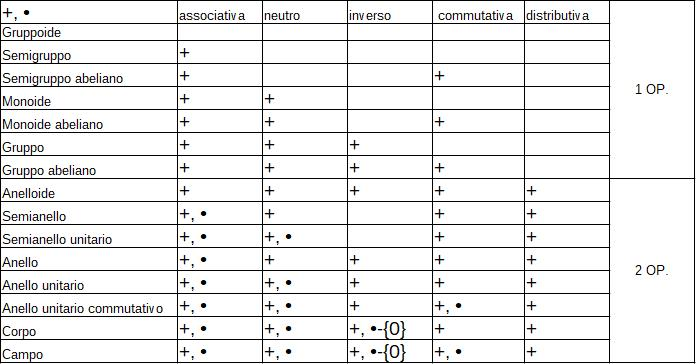
\includegraphics[scale=1]{strutture_algebriche.jpg}

\section{Numeri interi}
Per la somma l'insieme dei numeri interi gode delle seguenti proprietà:
\begin{enumerate}
    \item \textbf{commutativa}
    \[\forall a,b \in \mathbb{Z} \Rightarrow a+b =  b + a\]
    
    \item \textbf{associativa} \[\forall z_1,z_2,z_3 \in \mathbb{Z}\rightarrow (z_1 + z_2) + z_3 = z_1 + (z_2 + z_3)\]
    
    \item \textbf{elemento neutro} \[\forall z \in \mathbb{Z},\;\exists0\in \mathbb{Z}:z+0=0+z=z\]
    
    \item \textbf{elemento simmetrico} \[\forall z \in \mathbb{Z}\;\exists!(-z)\in\mathbb{Z}:z+(-z) = (-z) + z = 0\]
\end{enumerate}
Quando valgono le proprietà 2, 3 e 4 si dice che l'insieme ha una struttura di \textbf{gruppo}.
Alla luce di ciò, visto che vale anche la proprietà 1, l'insieme $\mathbb{Z}$ si dice che assume una struttura di gruppo commutativo o abeliano rispetto alla \textbf{somma}, $(\mathbb{Z}, +)$.

Per il prodotto, l'insieme dei numeri interi gode delle seguenti proprietà 

\begin{enumerate}
    \item \textbf{commutativa}
    \[\forall a,b \in \mathbb{Z} \Rightarrow a\cdot b =  b \cdot a\]
    
    \item \textbf{associativa} \[\forall z_1,z_2,z_3 \in \mathbb{Z}\rightarrow (z_1 \cdot z_2) \cdot z_3 = z_1 \cdot (z_2 \cdot z_3)\]
    
    \item \textbf{elemento neutro} \[\forall z \in \mathbb{Z},\;\exists 1\in \mathbb{Z}:z+1=1+z=z\]
    
    \item \textbf{distributiva (rispetto alla somma)} \[\forall a,bc, \in \mathbb{Z} \Rightarrow(a+b) \cdot c = a\cdot c + b \cdot c\]
\end{enumerate}
È importante notare che per $(\mathbb{Z,\cdot})$ non può esistere l'elemento simmetrico in quanto apparterrebbe ai numeri razionali $\mathbb{Q}$.\\
Alla luce di quanto detto sulle proprietà che valgono in $\mathbb{Z}$, possiamo dire che $(\mathbb{Z,+,\cdot})$ è un anello con unità commutativa.

\subsection{Validità della divisione}
\[\forall a,b \in \mathbb{Z},\,b\neq 0\,\exists! q,r\in \mathbb{Z}:a=b\,q +r,\;0\leq r<\abs{b}\]
(segue dimostrazione sull'esistenza di $q$ ed $r$).
\newpage
(segue dimostrazione dell'unicità di $q$ ed $r$).
\\ \vspace{300px}


\subsection{Divisori}
\begin{definizione} [Divisore]
Dati due numeri interi $a$ e $b$, si dice che $b$ divide $a$ (o $a$ è multiplo di $b$ o $b$ è divisore di $a$) e si scrive
\[b|a\]
se esiste $c\in \mathbf{Z}:a = bc$.
\end{definizione}
Possiamo inoltre osservare le seguenti:
\begin{itemize}
    \item $a|0$;
    \vspace{100px}
    \item $0|a\Rightarrow a = 0$;
    \vspace{100px}
    \item $b|a$, con $b\neq 0\Leftrightarrow$ il resto della divisione di $a$ per $b$ è $0$;
    \vspace{100px}
    \item $\forall a \in \mathbf{Z}, \pm 1,\pm a$ sono divisori di $a$, infatti $a = a\cdot 1 = (-a)\cdot(-1)$;
    \vspace{100px}
\end{itemize}
Sfruttando l'ultima osservazione, possiamo dare la seguente

\begin{definizione}[Divisori impropri]
Sia $a\in \mathbf{Z}$.\\
Allora $\pm 1, \pm a$ sono detti divisori \textbf{impropri} di $a$.\\
Di conseguenza, un divisore $b$ di $a$ tale che $b\neq \pm 1, \pm a$ è detto divisore proprio di $a$.
\end{definizione}

In merito ai divisori, possiamo adesso enunciare le seguenti 

\begin{proprieta}[Transitiva]
\[\forall b_1, b_2, b_3 \in \mathbf{Z}, b_1|b_2 \land b_2|b_3 \Rightarrow b_1 |b_3\]
(segue dimostrazione)\\
\vspace{100px}
\end{proprieta}

\begin{proprieta}
\[\forall b_1, b_2 \in \mathbf{Z}, b_1|b_2 \land b_2|b_1 \Rightarrow b_1 = \pm b_2\]
(segue dimostrazione)\\
\vspace{150px}
\end{proprieta}


\begin{proprieta}[\hypertarget{lemma1diofantee}{Compatibilità con somma e differenza}]
\[\forall b_1, b_2, b_3 \in \mathbf{Z}, b_1|b_2 \land b_1|b_3 \Rightarrow b_1 |(b_2 \pm b_3)\]
(segue dimostrazione)\\
\vspace{100px}
\end{proprieta}

Diamo la seguente
\begin{definizione}[Interi associati]
Dati due interi $a, b \in \mathbf{Z}$.\\
Allora, $a, b$ si diranno associati se $a|b$ e $b|a$ ossia se si dividono a vicenda; si scrive
\[a\sim b\]
\end{definizione}
\begin{osservazione}
\[a\sim b \Leftrightarrow a = \pm b\]
\end{osservazione}
\begin{osservazione}
In $\mathbf{Z}$ consideriamo la seguente relazione R: $a,b \in \mathbf{Z},\,aRb\Leftrightarrow a\sim b$.\\
Si verifica facilmente che R è una relazione d'equivalenza.
\end{osservazione}
\subsubsection{Numero primo}
Un numero $p$ si dice primo se ha come divisori soltanto $\pm 1$ e $\pm p$.\\
In altri termini se possiede soltanto divisori impropri.

\subsection{Massimo Comun Divisore}
\begin{definizione}[Massimo comun divisore]
Dati due numeri interi $a, b \in \mathbb{Z}$ si definisce massimo comun divisore di $a$ e $b$ un intero $d$ che soddisfa le seguenti proprietà:
\begin{itemize}
    \item $d$ è un divisore comune di $a$ e di $b$
    \[d|a \land d|b\]
\begin{domanda}
Come si traduce questa espressione in relazione alle proprietà dei divisori?\\
\vspace{100px}
\end{domanda}
    \item ogni altro divisore $d_0$ comune di $a$ e di $b$ è divisore di $d$
    \[d_0|a, d_0|b\Rightarrow d_0|d\]
\end{itemize}
\end{definizione}
\begin{osservazione}
Se d e d' sono due massimi comun divisori di $a$ e di$b$ allora sono necessariamente associati, ossia sono l'uno l'opposto dell'altro
\[d =\pm d'\]
 \end{osservazione}
\begin{domanda}
Come si spiega l'osservazione precedente?\\
\vspace{100px}
\end{domanda}

\begin{osservazione}
Si noti che si definisce {\color{red}{\textbf{il}}} massimo comun divisore di $a$ e di $b$ quello tra i due che è maggiore o uguale a zero.
\end{osservazione} 

\begin{domanda}
Quali conclusioni possiamo trarre dalla risposta alla domanda 5.2 e dall'osservazione 5.11?\\
\vspace{100px}
\end{domanda}

\begin{theorem}[Esistenza del Massimo Comun Divisore]
Dati due numeri interi $a, b \in \mathbf{Z}$ esiste sempre il loro massimo comun divisore, $d = (a, b)$ e si può scrivere nella forma 
\[d = ax + by\]
per opportuni $x, y \in \mathbf{Z}$
\end{theorem}
(segue dimostrazione)\\
\vspace{250px}
 

\begin{osservazione}
La scrittura
\[d = ax + by\]
è detta Identità di Bézout.\\
Si noti che tale espressione non è unica, infatti
\[1 = 3\cdot + (-4)\cdot 5 = (-2) \cdot 7 + 3\cdot 5\] 
\end{osservazione}

Ciò che quindi ci chiediamo è, dati due numeri interi $a,b\in \mathbf{Z}$
\begin{enumerate}
    \item Come determiniamo il MCD, d=(a,b)?
    \item Come determiniamo una identità di Bézout d = ax + by?
\end{enumerate}
Possiamo rispondere ad entrambe le domande mediante \textit{l'algoritmo Euclideo delle divisioni successive}.\\
Questo si basa sul seguente risultato:
\begin{proposizione}
Siano $a, b\in \mathbf{Z},b\neq 0$.\\
Sia $a = bq + r$, con $0\leq r < \abs{b}$, allora:
\[(a,b) = (b, r)\]
\end{proposizione}
(segue dimostrazione)\\
\vspace{150px}

\subsubsection{Algoritmo Euclideo delle divisioni successive}
L'algoritmo Euclideo consiste in una successione finita di divisioni euclidee in modo che il divisore e il resto, se non nullo, diventino rispettivamente il dividendo e il divisore della divisione successiva; il processo si arresta non appena si trova un resto non nullo.\\
Siano $a, b \in \mathbf{Z}$.\\
Se $b = 0$ si ha $(a, 0) = \abs{a} = a\cdot (\pm 1) + 0\cdot y$.\\
Analogamente, se $a = 0$ si ha $(0, b) = \abs{b} = 0\cdot x + b\cdot (\pm 1)$.
Inoltre $(a, b) = (\pm a, \pm b)$ e $(a, b)=(b, a)$.\\
Per cui possiamo supporre $a\geq b > 0$.\\
In altre parole, in metodo è il seguente
\begin{itemize}
    \item[] $a = b\,q_1 + r_1\hspace{10px}0\leq r_1 < b$
    \item[] $b = r_1\,q_2 + r_2\hspace{10px}0\leq r_2 < r_1$
\end{itemize}
\hspace{30px}\vdots
\begin{itemize}
    \item[] $r_{k-2} = r_{k-1}\,q_k + r_k\hspace{10px}0\leq r_k < r_{k-1}$
    \item[] $r_{k-1} = r_k\,q_{k+1} + r_2\hspace{10px}0\leq r_k < r_{k-1}$
\end{itemize}
$r_k$, ovvero l'ultimo resto non nullo è il massimo comun divisore di $a$ e $b$.\\
$r_k | r_{k-1} \Rightarrow r_k|r_{k-1}\cdot q_k + r_k \Rightarrow r_k | r_{k-2} \Rightarrow r_k | r_{k-3} \Rightarrow \hdots \Rightarrow r_k|a \Rightarrow r_k |b$.\\
Poiché $r_k$ è il massimo comun divisore se\\
$d'|a \land d'|b \Rightarrow d'|r_k$

\begin{esempio}[(72, 22) = ?]
\begin{itemize}
    \item[] $72 = 22 \cdot 3 + 6$
    \item[] $22 = 6 \cdot 3 + 4$
    \item[] $6 = 4 \cdot 1 + 2$
    \item[] $4 = 2 \cdot 2 + 0$
\end{itemize}
Dunque $(72, 22) = 2$.\\
Come detto, però, possiamo, attraverso il metodo euclideo delle divisioni successive, determinare una identità di Bézout.\\
Per il teorema sull'esistenza del Massimo Comun Divisore si ha che esistono due interi $x, y$ tali che
\[2 = 72 \cdot x + 22 \cdot y\]
determiniamo $x$ e $y$.\\
Visto che
\begin{itemize}
    \item[] $72 = 22 \cdot 3 + 6$
    \item[] $22 = 6 \cdot 3 + 4$
    \item[] $6 = 4 \cdot 1 + 2$
    \item[] $4 = 2 \cdot 2 + 0$
\end{itemize}
Allora\\
\vspace{10px}
$ \left.
  \begin{cases}
    2 = 6 - 4 \cdot(1)\\
    4 = 22 - 6 \cdot(3)\\
  \end{cases}
  \right\} = 2 = 6 - (22 -  6\cdot 3)\cdot (1) = 6 + 6\cdot 3 - 22 = 6(1+3) - 22 = 6 \cdot 4 - 22
$\\
$2 = 6 - 4 = 6 - 22 + 6\cdot 3 = 6 \cdot 4 - 22 = (72 - 22 \cdot 3) \cdot 4 - 22 = 72 \cdot 4 - 22 \cdot 12 - 22 = 72 \cdot 4 - 22 \cdot 13$
in definitiva, allora
\[2 = 72 \cdot 4 + 22 \cdot (-13)\]
\end{esempio}


\subsubsection{Coprimi}
Due numeri interi $a$ e $b$ si dicono coprimi se il loro massimo comun divisore è 1, ossia (a, b) = 1.\\
Diamo, inoltre, il seguente
\begin{criterio}
Dati $a, b \in \mathbf{Z}$, allora, $a$ e $b$ sono coprimi se e soltanto se 1 si può scrivere come loro combinazione lineare a coefficienti interi
\[(a, b) = 1 \Leftrightarrow 1 = a\cdot x + b \cdot y,\hspace{10px}x, y \in \mathbf{Z}\]
\end{criterio}
(segue dimostrazione dal t. es. mcd)\\
\vspace{100px}
\begin{cons}
\begin{enumerate}
    \item due interi consecutivi sono coprimi
    \[(a, a+1) = 1, \forall a\in \mathbf{Z}\]
    \item dividendo due interi per il loro massimo comun divisore si ottengono interi coprimi
    \[\Bigl(\frac{a}{(a, b)}, \frac{b}{(a, b)} \Bigr) = 1\]
\end{enumerate}
\end{cons}

\begin{esercizio}
Si dimostrino entrambe le conseguenze precedenti.
\end{esercizio}
\vspace{100px}

\begin{proposizione}
Siano $a, p \in \mathbf{Z},\,p$ primo.\\
Se $p\not{|}a|\Rightarrow (p, a) = 1$ 
\end{proposizione}
\begin{esercizio}
Si dimostri la proposizione.
\end{esercizio}
\vspace{100px}

\begin{proposizione}
Se un intero divide un prodotto di interi ed è coprimo con uno dei due fattori, allora divide l'altro, ossia:
\[\forall a,b,c \in \mathbf{Z}, a|bc, (a, b) = 1 \Rightarrow a|c\]
\end{proposizione}
\begin{esercizio}
Si dimostri la proposizione.
\end{esercizio}
\vspace{100px}

\begin{proposizione}
Siano $a, b, m\in \mathbf{Z}$ e $(a, b) = 1$, allora
\[a|m, b|m, (a, b)=1 \Rightarrow ab|m\]
\end{proposizione}
\begin{esercizio}
Si dimostri la proposizione.
\end{esercizio}
\vspace{100px}


\subsection{Minimo comune multiplo}
\begin{definizione}

\end{definizione}
Dati due numeri interi $a, b \in \mathbf{Z}$ si definisce minimo comune multiplo di $a$ e di $b$, e si denota con $\big[a,b\big]$, l'intero positivo $m$ che soddisfa le seguenti proprietà:
\begin{itemize}
    \item $m$ è un multiplo comune di $a$ e di $b$:
    \[a|m \land b|m\]
    \item ogni altro multiplo $m_0$ comune di $a$ e di $b$ è multiplo di $m$:
    \[a|m_0\land b|m_0 \Rightarrow m|m_0\]
\end{itemize}
\begin{osservazione}
Come per il massimo comun divisore si dimostra che se $m$ ed $m'$ sono due minimi comuni multipli di $a$ e di $b$ allora sono associati, ossia $m = \pm m'$.
\end{osservazione}





\begin{theorem}
Dati $a, b \in \mathbf{Z}$, allora $\exists\big[a, b\big]$ e 
\[(a, b)\big[a, b\big] = \abs{ab}\]
\end{theorem}
\begin{esempio}
\[\big[72, 22\big] = \frac{\abs{72\cdot 22}}{(72, 22)} = \frac{72\cdot 22}{2} = 72     \cdot 11 = 792\]
\end{esempio}

\begin{esercizio}
Si dimostri la proposizione.
\end{esercizio}
\vspace{200px}

\subsection{Teorema fondamentale dell'aritmetica}
L'importanza della classe dei numeri primi consiste nel fatto che ogni numero naturale maggiore di 1 può essere espresso come prodotto di primi.\\
Questa affermazione, a prima vista così ovvia, è nota come teorema fondamentale dell'aritmetica, diamo allora il seguente:
\begin{theorem}[Teorema fondamentale dell'aritmetica]
Ogni naturale $n>1$ si può scrivere come prodotto di primi
\[n = p_1p_2\hdots p_k\]
con $p_i$ primo $\forall i= 1,...,k$.
Inoltre, tale fattorizzazione è \textbf{unica} a meno dell'ordine dei fattori, ossia se esistono due fattorizzazioni
\[n = p_1p_2\hdots p_k = q_1q_2\hdots q_k\]
con $p_i$ e $q_j$ primi, allora $k=h$ e riordinando opportunamente i fattori si ha: $p_1=q_1,p_2=q_2\hdots p_k=q_k$
\end{theorem}
\begin{esercizio}
Si dimostri l'esistenza di tale fattorizzazione (insieme non vuoto).
\end{esercizio}
\vspace{200px}
\begin{esercizio}
Si dimostri l'unicità di tale fattorizzazione (induzione).
\end{esercizio}
\vspace{200px}

\begin{theorem}[Esistenza di infiniti numeri primi]
Esistono infiniti numeri primi
\end{theorem}
\begin{esercizio}
Si dimostri il teorema per assurdo.
\end{esercizio}
\vspace{200px}


\begin{theorem}[$\sqrt{p}$ non è razionale]
Sia $p>1$ un numero primo.\\
Allora $\sqrt{p}$ non è un numero razionale.
\end{theorem}
\begin{esercizio}
Si dimostri il teorema per assurdo.
\end{esercizio}
\vspace{200px}




\subsection{Esercizi}
\begin{esercizio}
Calcolare il massimo comun divisore tra $1547$ e $560$.\\
Si scriva, inoltre, l'identità di Bézout.
\end{esercizio}
\vspace{150px}

\begin{esercizio}
Calcolare il massimo comun divisore tra $-44880$ e $5292$.\\
Si scriva, inoltre, l'identità di Bézout.
\end{esercizio}
\vspace{150px}


\section{Congruenze}
\subsection{Congruenze in Z}
\begin{definizione}
Sia $n$ un intero fissato.\\
Si dice che $a, b \in \mathbf{Z}$ sono congruenti modulo $n$ e si scrive
\[a\equiv b (mod n)\]
se $n$ divide $a-b$, in altri termini, se esiste un intero $k \in \mathbf{Z}$ tale che $kn = a-b$.
\end{definizione}
\textbf{Si noti} che ciò definisce una relazione binaria su $Z$, detta, appunto, congruenza modulo $n$.

\begin{proposizione}[La congruenza modulo n è una relazione di equivalenza]
\end{proposizione}
\begin{esercizio}
Si dimostri la proposizione precedente.
\end{esercizio}
\vspace{150px}

\begin{definizione}[Classe di resto]
Per ogni $a \in \mathbf{Z}$, la classe di equivalenza di $a$ rispetto alla congruenza modulo $n$ si chiama classe di congruenza di $a$ modulo $n$ (o \textbf{classe di resto} di $a$ modulo $n$) e si indica con $\big[a\big]_n$.\\
Inoltre, l'insieme quoziente di $\mathbf{Z}$ rispetto alla congruenza modulo $n$ si denota con il simbolo $\mathbf{Z}_n$.
\end{definizione}

\begin{esempio}

\end{esempio}
Consideriamo ora la congruenza modulo 2 e siano $a, b \in \mathbf{Z}$.
Allora
\[a\equiv_2 b \Leftrightarrow a-b\;\;\text{è pari}\]
ciò avviene se $a,b$ sono entrambi pari o entrambi dispari.\\
Quindi le classi di congruenza modulo 2 sono esattamente 2: una è l'insieme dei numeri pari, l'altra l'insieme dei numeri dispari.\\
La prima è la classe di congruenza di 0, l'altra la classe di congruenza di 1; quindi, in definitiva, si ha che
\[\mathbf{Z}_2 = \{\big[0\big]_2, \big[1\big]_2\}\]
Possiamo allora, in generale, enunciare la seguente
\begin{proposizione}[Cardinalità di $\mathbf{Z}_n$]
Per ogni intero positivo $n$, $\mathbf{Z}_n$ ha n elementi e, precisamente,
\[\mathbf{Z}_n =  \{\big[0\big]_n, \big[1\big]_n,...,\big[n-1\big]_n\}\]
\end{proposizione}
\textbf{Si noti} che gli elementi $0, 1,...,n-1$ si dicono i \textit{rappresentanti canonici} della congruenza modulo n.\\
Se $a_0, a_1,...,a_{n-1}\in \mathbf{Z}$ sono tali che $\mathbf{Z_n} = \{\big[a_0\big]_n, \big[a_1\big]_n,...,\big[a_{n-1}\big]_n\}$ è un sistema completo di rappresentanti per la congruenza modulo $n$.
\begin{esempio}

\end{esempio}
Si consideri $\mathbf{Z}_3 = \{\big[0\big]_3, \big[1\big]_3,\big[2\big]_3\}$.\\
Allora un sistema completo di rappresentanti per la congruenza modulo $3$ è $\{3, 4, 5\}$, o anche $\{330, 3001, 12362\}$




\begin{esercizio}
Si dimostri la proposizione precedente.
\end{esercizio}
\vspace{150px}

\begin{proposizione}[Compatibilità della congruenza rispetto alla somma e al prodotto]
Siano $a, a', b, b'\in \mathbf{Z}$ tali che $a\equiv_n a'$ e $b\equiv_n b'$, allora
\begin{enumerate}
    \item $a+b \equiv_n a'+b'$;
    \item $ab \equiv_n a'b'$.
\end{enumerate}
\end{proposizione}
\begin{esercizio}
Si dimostri la proposizione precedente.
\end{esercizio}
\vspace{150px}

\begin{osservazione}

\end{osservazione}
Si noti che le proprietà 1 e 2 della proposizione precedente si possono riassumere dicendo che la congruenza modulo $n$ è \textbf{compatibile} rispetto alla somma e al prodotto.\\
Queste proprietà consentono di dotare l'insieme $\mathbf{Z}_n$ di una struttura di anello, definiamo su di esso, allora, le seguenti operazioni
\begin{itemize}
    \item \textbf{Somma:} $\forall a, b \in \mathbf{Z}, \big[a\big]_n + \big[b\big]_n = \big[a+b\big]_n$;
    \item \textbf{Prodotto:} $\forall a, b \in \mathbf{Z}, \big[a\big]_n \cdot \big[b\big]_n = \big[a\cdot b\big]_n$.
\end{itemize}
Queste definizioni sono ben poste, ossia la classe di congruenza a secondo membro non dipende dalla scelta dei rappresentanti $a$ e $b$ nelle classi di congruenza a primo membro: infatti, in base alla proposizione 6.6 $\big[a\big]_n = \big[a'\big]_n$ e $\big[b\big]_n = \big[b'\big]_n$, allora
\begin{itemize}
    \item[] $\big[a\big]_n + \big[b\big]_n = \big[a+b\big]_n$;
    \item $\big[a\big]_n \cdot \big[b\big]_n = \big[a\cdot b\big]_n$.
\end{itemize}
A parole, la definizione significa che per sommare due classi si sceglie il rappresentante di ciascuna classe, si somma (in base all'usuale somma di numeri interi) e si calcola la classe del risultato.\\
\textbf{Si noti} che il simbolo a destra dell'uguaglianza rappresenta l'usuale somma di numeri interi, quello a sinistra rappresenta la nuova operazione fra classi che si vuole definire.

\subsubsection{Esercizi}
\begin{esercizio}
Si risolva la congruenza $27 \equiv_5 2$ e si indichi la classe di resto.
\end{esercizio}
\vspace{150px}

\begin{esercizio}
Si risolva la congruenza $37 \equiv_8 13$ e si indichi la classe di resto.
\end{esercizio}
\vspace{150px}


\begin{esercizio}
Si risolva la congruenza $143 \equiv_{12} 23$ e si indichi la classe di resto.
\end{esercizio}
\vspace{150px}

\begin{esercizio}
Si calcoli $\big[124\big]_4$
\end{esercizio}
\vspace{100px}

\begin{esercizio}
Si calcoli $\big[25\big]_3$
\end{esercizio}
\vspace{100px}

\begin{esercizio}
Si calcoli $\big[37\big]_5$
\end{esercizio}
\vspace{100px}

\begin{esercizio}
Si calcoli $\big[210\big]_6$
\end{esercizio}
\vspace{100px}

\begin{esercizio}
Si calcoli $\big[27\big]_3$
\end{esercizio}
\vspace{100px}

\begin{esercizio}
Si calcoli $\big[315\big]_{10}$
\end{esercizio}
\vspace{100px}


\subsection{Equazioni Diofantee}
Come visto precedentemente (\hyperlink{lemma1diofantee}{qui}), possiamo enunciare il seguente
\begin{lemma}
Siano $d, a, b \in \mathbf{Z}$.\\
Se $d|a$ e $d|b \Rightarrow d|ax + by\;\forall x,y \in \mathbf{Z}$
\end{lemma}
\begin{esercizio}
Si dimostri il lemma precedente.
\end{esercizio}
\vspace{150px}

\begin{cons}
Se $d = (a, b) \Rightarrow d|ax + by\; \forall x, y \in \mathbf{Z}$.
\end{cons}
\begin{definizione}
Siano $a,b, c \in \mathbf{Z}.$\\
Una equazione nella forma $ax + by = c$ nelle variabili $x, y$ si dice equazione diofantea.
\end{definizione}
Uno dei problemi che potremmo ritrovarci a risolvere, ad esempio, è $4x + 5y = 1$ che ammette soluzioni intere $x = -1, y = 1$ ma anche $x=4, y = -3$.\\
In generale, allora, possiamo dare la seguente
\begin{proposizione}
Condizione necessaria e sufficiente affinché l'equazione diofantea $ax + by = c,\;a,b,c \in \mathbf{Z}$ ammetta soluzione è che $MCD(a, b) = d|c$, ossia
\[\exists\;sol\;ax + by = c \Leftrightarrow MCD(a, b) = d|c \Leftrightarrow c = d\cdot t\]
\end{proposizione}
\begin{esempio}
\end{esempio}
Ad esempio, l'equazione $3x + 7y = 2$ ammette soluzione, poiché $(3, 7) = 1$ e $1|2$.\\
Osserviamo che, allora, $1 = 3(-2) + 7(1)$ da cui, moltiplicando per $2$ entrambi i membri si ha
\[2 = 3(-4) + 7(2)\]
\textbf{Si noti} però, che come detto la soluzione $(-4, 2)$ è \textbf{una} soluzione e quindi non è unica, infatti anche $(10, -4)$ è soluzione.
\begin{esercizio}
Si dimostri la proposizione precedente.
\end{esercizio}
\vspace{200px}

\begin{osservazione}[Algoritmo per la risoluzione]
La dimostrazione della proposizione precedente, ci offre un metodo per determinare una soluzione dell'equazione $ax + by = c$.\\
Infatti, basta esprimere il $MCD(a, b) = d$ come $d = a\cdot \alpha + b \cdot \beta$ e allora, poiché $d|c\Rightarrow c = d\cdot h = (a\alpha + b \beta) h= a(\alpha h) + b(\beta h)$ quindi la soluzione è la coppia
\[x = \alpha h,\;y = \beta h\]
\end{osservazione}

\begin{proposizione}
Sia $(x, y)$ una soluzione intera dell'equazione $ax + by = c$, allora tutte le soluzioni sono del tipo $(x', y')$ dove
\[x' = x - \frac{b}{d}t,\;y' = y - \frac{a}{d}t\;\forall t \in \mathbf{Z}\]
dove $d = MCD(a, b)$.
\end{proposizione}

\subsubsection{Esercizi}
\begin{esercizio}
Determinare una soluzione, se esiste, dell'equazione $153x + 45y = 18$
\end{esercizio}
\vspace{150px}



\begin{esercizio}
Determinare una soluzione, se esiste, dell'equazione $7x + 13y = -5$
\end{esercizio}
\vspace{150px}


\subsection{Equazioni congruenziali}
\begin{definizione}
Sia $n$ un intero positivo.\\
Si dice congruenza lineare (modulo n) il problema di trovare tutti i numeri interi $x$ che soddisfano una relazione di congruenza della forma
\[ax \equiv_n b,\;a,b\in \mathbf{Z}, a\neq 0\]
\end{definizione}

\begin{proposizione}[Risolubilità di congruenze lineari]
Sia $n$ un intero positivo e siano $a, b \in \mathbf{Z}$, dove $a\neq 0$.\\
Sia, inoltre, $d = MCD(a, n)$, allora la congruenza lineare
\[ax \equiv_n b\]
ammette soluzione se e solo se $d|b$.\\
In tal caso, detta $x_0$ una soluzione particolare, le soluzioni sono tutti e soli i numeri interi
\[x_k = x_0 + \frac{n}{d}k\]
\end{proposizione}
\begin{esercizio}
Si dimostri la proposizione precedente.
\end{esercizio}
\vspace{200px}
\begin{osservazione}
Supponiamo, allora, che la congruenza lineare
\[ax \equiv_n b\]
abbia soluzione, ossia che $d|b$.
Allora, questa sarà equivalente alla congruenza lineare
\[\frac{a}{d}x \equiv_\frac{n}{d} \frac{b}{d}\]
ove $\frac{a}{d}$ e $\frac{n}{d}$ sono coprimi.
\end{osservazione}

Seppure, allora, l'introduzione delle equazioni diofantee tra le congruenze lineari e le equazioni congruenziali possa sembrare anacronistica, ciò non è vero.\\
Infatti, il problema della ricerca di una congruenza lineare in una indeterminata è equivalente a quello della ricerca delle soluzioni di una equazione diofantea in due indeterminate.\\
Poiché $x'$ è una soluzione di $aX \equiv_n b$ se, e soltanto se, esiste $y'\in \mathbf{Z}$ tale che $ax' - b = ny'$, ovvero se, e soltanto se, $(x', y')$ è soluzione dell'equazione diofantea
\[ax - ny = b\]
Una soluzione, allora, può essere esplicitamente trovata riducendo il problema alla risoluzione dell'equazione diofantea nelle indeterminate $x$ ed $y$, ovvero calcolando i coefficienti della relazione di Bézout che esprime $d := MCD(a, n)$, ricorrendo all'algoritmo euclideo delle divisioni successive.

\subsubsection{Esercizi}
\begin{esercizio}
Si risolva l'equazione congruenziale $15x \equiv_{21} 12$.
\end{esercizio}
\vspace{150px}


\begin{esercizio}
Si risolva l'equazione congruenziale $7x \equiv_5 3$.
\end{esercizio}
\vspace{150px}

\begin{esercizio}
Si risolva l'equazione congruenziale $5x \equiv_{11} 5$.
\end{esercizio}
\vspace{150px}

\begin{esercizio}
Si risolva l'equazione congruenziale $7x \equiv_{10} 4$.
\end{esercizio}
\vspace{150px}

\begin{esercizio}
Si risolva l'equazione congruenziale $21x \equiv_5 6$.
\end{esercizio}
\vspace{150px}

\begin{esercizio}
Si risolva l'equazione congruenziale $13x \equiv_{12} 11$.
\end{esercizio}
\vspace{150px}

\begin{esercizio}
Si risolva l'equazione congruenziale $259x \equiv_{11} 16$.
\end{esercizio}
\vspace{150px}

\begin{esercizio}
Si risolva l'equazione congruenziale $7x \equiv_{256} 16$.
\end{esercizio}
\vspace{150px}


\begin{esercizio}
Si risolva l'equazione congruenziale $73x \equiv_{35} -101$.
\end{esercizio}
\vspace{150px}



\subsection{Teorema cinese del resto}
\begin{theorem}
Condizione sufficiente affinché il sistema di congruenze
\[\begin{cases}
x\equiv_{n_1} a_1\\
x\equiv_{n_2} a_2\\
\vdots\\
x\equiv_{n_s} a_s
\end{cases}
\]
ammetta soluzioni è che i moduli siano a due a due coprimi, ovvero che $\forall i\neq j \Rightarrow (n_i, n_j) = 1$.
\end{theorem}
\begin{osservazione}
Si noti che se $x_0$ è una soluzione, \textbf{tutte} le soluzioni di tale sistema saranno date da:
\[x = x_0 + h (n_1\cdot n_2\hdots n_s),\; h\in \mathbf{Z} \]
\end{osservazione}
\begin{esercizio}
Si dimostri l'esistenza della soluzione.
\end{esercizio}
\vspace{200px}

\begin{esercizio}
Si dimostri l'unicità della soluzione.
\end{esercizio}
\vspace{200px}



\subsubsection{Esercizi}
\begin{esercizio}
Determinare se esiste la soluzione del seguente sistema lineare
\[\begin{cases}
x\equiv_{4} 2\\
x\equiv_{6} 7
\end{cases}
\]
\end{esercizio}
\vspace{200px}


\subsection{Sistemi di congruenze}
Consideriamo adesso un sistema di congruenze generico del tipo
\[(1)\; \begin{cases}
a_1x\equiv_{n_1} b_1\\
a_2x\equiv_{n_2} b_2\\
\vdots\\
a_sx\equiv_{n_s} b_s
\end{cases}
\]
in cui supporremo $(n_i, n_j) = 1$, per $i\neq j$.\\
Allora, una soluzione di tale sistema è un intero che soddisfa contemporaneamente tutte le congruenze del sistema, segue dunque che il sistema sarà compatibile $\Leftrightarrow (a_i, n_i)|b_i\;\forall i = 1,...,s$.\\
La risoluzione del sistema $(1)$ equivale a risolvere un sistema del tipo
\[\begin{cases}
x\equiv_{n_1'} c_1\\
x\equiv_{n_2'} c_2\\
\vdots\\
x\equiv_{n_s'} c_s
\end{cases}
\]
con $(n_i', n_j') = 1$.\\
Infatti, se $(1)$ ammette soluzione allora $d_i = MCD(a_i, n_i)| b_i,\;\forall i=1,...,s$.\\
Dividendo la $i-$esima congruenza per $d_i =MCD(a_i, n_i')$ si ottiene un sistema equivalente
\[\begin{cases}
a_1'x\equiv_{n_1'} b_1'\\
a_2'x\equiv_{n_2'} b_2'\\
\vdots\\
a_s'x\equiv_{n_s'} b_s'
\end{cases}
\]
dove $a_k' = \frac{a_k}{d_k}, b_k' = \frac{b_k}{d_k}, n_k' = \frac{n_k}{d_k}$.\\
Poiché $(a_k', n_k') = \big(\frac{a_k}{d_k}, \bigr) = 1\Rightarrow $ ogni congruenza ammette soluzione unica $c_i (mod\;n_i')$ quindi
\[\begin{cases}
x\equiv_{n_1'} c_1\\
x\equiv_{n_2'} c_2\\
\vdots\\
x\equiv_{n_k'} c_k
\end{cases}
\]



\subsubsection{Esercizi}

\begin{esercizio}
Scrivere un sistema di tre equazioni congruenziali che non ammetta soluzioni (intere) sebbene le sue singole equazioni (separatamente) ne ammettano.
\end{esercizio}
\vspace{200px}

\begin{esercizio}
Determinare se esiste la soluzione del seguente sistema lineare
\[\begin{cases}
3x\equiv_{5} 3\\
5x\equiv_{7} 3
\end{cases}
\]
\end{esercizio}
\vspace{200px}

\begin{esercizio}
Determinare se esiste la soluzione del seguente sistema lineare
\[\begin{cases}
7x\equiv_{4} 5\\
21x\equiv_{5} 2
\end{cases}
\]
\end{esercizio}
\vspace{200px}

\begin{esercizio}
Calcolare tutte le soluzioni del sistema di equazioni congruenziali seguente:
\[\begin{cases}
21x\equiv_{4} -93\\
-11x\equiv_{7} \\
6178x\equiv_{3} 983\\
71x\equiv_{5} 52
\end{cases}
\]
\end{esercizio}
\vspace{200px}


\begin{esercizio}
Calcolare tutte le soluzioni del sistema di equazioni congruenziali seguente:
\[\begin{cases}
79x\equiv_{8} 91\\
-81x\equiv_{7} -129\\
39x\equiv_{15} 132
\end{cases}
\]
\end{esercizio}
\vspace{200px}


\begin{esercizio}
Calcolare tutte le soluzioni del sistema di equazioni congruenziali seguente:
\[\begin{cases}
17x\equiv_{5} -105\\
-55x\equiv_{3} 11\\
23x\equiv_{7} 36
\end{cases}
\]
\end{esercizio}
\vspace{200px}

\begin{esercizio}
Verificare che il seguente sistema di equazioni congruenziali
\[\begin{cases}
3x\equiv_{10} 7\\
3x\equiv_{5} 2
\end{cases}
\]
ha esattamente dieci soluzioni $x$ tali che $0\leq x \leq 100$
\end{esercizio}
\vspace{200px}



\subsection{Calcolo combinatorio}
\subsubsection{Fattoriale}
Sia $n$ un numero naturale, il fattoriale $n!$ è dato da
\[n! = n\cdot (n-1)\cdot(n-2)\cdot\hdots\cdot2\cdot1\]
\subsubsection{Applicazioni biiettive di un insieme}
Sia $A$ un insieme di cardinalità $\abs{A} = n$.\\
Il numero di applicazioni biiettive da $A$ in $A$ è uguale a $n!$.
\subsubsection{Permutazione}
Una permutazione è un'applicazione biunivoca di un insieme in sé stesso.
\subsubsection{Coefficiente binomiale}
Sia $A$ un insieme di cardinalità $\abs{A} = n$.\\
Tramite il coefficiente binomiale $\binom{n}{k}$ si può trovare il numero di tutti i possibili sottoinsiemi di $A$ di cardinalità $k$ fissata e si esprime nel seguente modo
 \[
       \binom{n}{k} = \frac{n!}{k!(n-k)!}
    \]
(segue dimostrazione)
\\ \vspace{150px}
Il coefficiente binomiale gode della seguenti proprietà:
\begin{itemize}
    \item  \[
       \binom{n}{0} = \frac{n!}{0!(n-0)!} = \frac{n!}{1\cdot n!} = 1
    \]
    \item  \[
       \binom{n}{n} = \frac{n!}{n!(n-n)!} = 1
    \]
    \item  \[
       \binom{n}{1} = \frac{n!}{k!(n-k)!} = \frac{n\cdot (n-1)!}{(n-1)!} = n
    \]
    \item  \[
       \binom{n}{k} = \binom{n-1}{k} + \binom{n-1}{k-1}
    \]                
\end{itemize}
\subsubsection{Binomio di Newton}
Il binomio di Newton permette di calcolare una qualsiasi potenza di binomio tramite la formula
\[(x+y)^n = \sum_{k=0}^n \binom{n}{k} \cdot x^{n-k}\cdot y^k\]
(segue dimostrazione, similitudine con triangolo di tartaglia)
\\ \vspace{300px}




\subsection{Teoremi di Eulero e Fermat}
\begin{lemma}[Congruenza di potenza di binomio]
Sia p un numero primo.\\
Per ogni $x, y \in \mathbf{Z}: (x+y)^p = x^p + y^p\;(mod\;p)$.
\end{lemma}
\begin{esercizio}
Si dimostri il lemma precedente.
\end{esercizio}
\vspace{150px}

\begin{theorem}[Piccolo teorema di Fermat]
Sia $p$ un numero primo, allora, per ogni $a\in \mathbf{Z}$,
\[a^p \equiv a\;(mod\,p)\]
\end{theorem}
\begin{esercizio}
Si dimostri il teorema precedente.
\end{esercizio}
\vspace{150px}


\begin{corollario}
Siano $a, p \in\mathbf{Z}$ con $(a, p) = 1$, se $p$ è primo, allora
\[a^{p-1} \equiv_p 1\]
\end{corollario}
\begin{esercizio}
Si dimostri il corollario precedente.
\end{esercizio}
\vspace{150px}
Diamo ora la seguente
\begin{definizione}[Funzione di Eulero]
Per ogni $n\geq 1$, si chiama funzione di Eulero l'applicazione (o funzione)
\[\varphi: \mathbf{N} \to \mathbf{N}: \varphi(1) = 1\]
e per ogni $n>1, \varphi(n)$ è il numero di interi positivi minori di $n$ e primi con $n$ e $\varphi(1) = 1$.
\end{definizione}

\begin{esempio}

\end{esempio}
\begin{itemize}
    \item $\varphi(2) = 1$;
    \item $\varphi(3) = 2$ perché $1,2$ sono gli interi positivi minori di $3$ e primi con 3;
    \item $\varphi(20) = 8$ perché gli interi positivi minori di 20 e primi con 20 sono: $1, 3, 7, 9 11, 13, 17, 19$.
\end{itemize}
Se però volessimo calcolare $\varphi(1320)$ ci troveremmo in difficoltà in quanto non è semplice trovare il numero dei naturali minori di $1320$ e primi con $1320$.\\
Per calcolare la funzione di Eulero di un dato numero intero $n$ ci vengono in aiuto alcune proprietà della funzione di Eulero.\\
La proprietà fondamentale della funzione di Eulero è di essere moltiplicativa.

\begin{lemma}
Siano $m, n\in \mathbf{N}$ tali che $(m, n) = 1$, allora $\varphi(m\cdot n) =\varphi(m)\varphi(n) $
\end{lemma}

\begin{lemma}
Siano $p\in \mathbf{N}$ un numero primo.\\
Allora:
\begin{enumerate}
    \item $\varphi(p) = p-1$;
    \item $\forall k \in \mathbf{N}, \varphi(p^k) = p^k - p^{k-1}$;
\end{enumerate}
\end{lemma}
\begin{esercizio}
Si dimostri il punto 2.
\end{esercizio}
\vspace{150px}
Quindi, dai lemmi precedenti si ha la seguente
\begin{proposizione}
Se $n = p_1^{k_1} \hdots p_r^{k_r}$ è la fattorizzazione di $n$ come prodotto di potenze di numeri distinti, allora
\[\varphi(n) = \varphi(p_1^{k_1} \hdots p_r^{k_r}) = \varphi(p_1^{k_1})\hdots \varphi(p_r^{k_r}) = p_1^{k_1}-p_1^{k_1-1}\hdots p_r^{k_r}-p_r^{k_r-1}\]
\end{proposizione}
\begin{esempio}

\end{esempio}
\[\varphi(234) = \varphi(2\cdot 3^2 \cdot 13) = \varphi(2) \cdot\varphi(3^2)\cdot\varphi(13) = 1\cdot (3^2-39)\cdot 12 = 1\cdot 6\cdot 12 = 72\]
Possiamo quindi enunciare il seguente teorema che non è possibile dimostrare con le conoscenze acquisite fino a questo momento ma verrà dimostrato in seguito ad alcuni risultati sui gruppi.

\begin{theorem}[Teorema di Eulero]
Sia $n\geq 2$ e sia $a\geq 2$ tale che $(a,n) = 1$, allora
\[a^{\varphi(n)}\equiv_n 1\]
\end{theorem}
\begin{corollario}
Se $n=p$ è un primo, si ottiene allora
\[a^{p-1} \equiv_p 1\]
\end{corollario}
\begin{osservazione}
Ogni numero intero, nella rappresentazione decimale, si rappresenta nella forma
\[a_n a_{n-1} a_{n-2}\hdots a_{1} a_{0}\]
con $0\leq a_i\leq 9.$\\
Tale numero deve intendersi come
\[a_n a_{n-1} a_{n-2}\hdots a_{1} a_{0} = a_n\cdot 10^n+ a_{n-1}\cdot 10^{n-1}+\hdots+ a_{1}\cdot 10 +a_{0}\]
\end{osservazione}

\begin{criterio}[Ultime cifre di un numero $a\in \mathbf{Z}$]
In generale volendo conoscere le ultime $n$ cifre di un numero $a\in \mathbf{Z}$ basta risolvere la congruenza $a\equiv x\,(mod\;10^n)$
\end{criterio}

\subsubsection{Esercizi}
\begin{esercizio}
Si calcolino le ultime due cifre di $n = 81^{82}$.
\end{esercizio}
\vspace{150px}

\subsubsection{Esercizi}
\begin{esercizio}
Si calcolino le ultime tre cifre di $n= 7^{827}$.
\end{esercizio}
\vspace{150px}

\subsubsection{Esercizi}
\begin{esercizio}
Si calcolino le ultime due cifre di $n = 47913^{6403}$.
\end{esercizio}
\vspace{150px}

\subsection{Criteri di divisibilità}
Si consideri un numero $z\in \mathbb{Z}$ di cifre $a_n a_{n-1} a_{n-2}\hdots a_2a_1a_0$, è possibile rappresentare quest'ultimo come
\[z = a_0 + a_1\cdot 10 + a_2\cdot 10^2+\hdots+a_{n-2}\cdot 10^{n-2} + a_{n-1}\cdot 10^{n-1}+a_n \cdot 10^n\]

\subsubsection{Divisibilità per 2}
Un numero è divisibile per 2 se la sua ultima cifra è divisibile per 2.
(segue dimostrazione)
\\ \vspace{300px}
\subsubsection{Divisibilità per 5}
Un numero è divisibile per 5 se la sua ultima cifra è divisibile per 5.
(segue dimostrazione analoga a quella della divisibilità per 2)
\\ \vspace{300px}
\subsubsection{Divisibilità per 3}
Un numero è divisibile per 3 se la somma delle sue cifre è divisibile per 3.
(segue dimostrazione)
\\ \vspace{300px}
\subsubsection{Divisibilità per 11}
Un numero è divisibile per 11 se la somma delle sue cifre pari meno la somma delle sue cifre dispari è divisibile per 11.
\[11| a_0-a_1+a_2-a_3+\hdots +(-1)^n a_n\]
(segue dimostrazione)
\\ \vspace{300px}





\section{Teoria dei Gruppi}
\begin{definizione}[Operazione binaria]
Sia $X$ un insieme non vuoto, si dice allora operazione (binaria) su X ogni applicazione
\[f: X \cross X \to X\]
\end{definizione}
Diamo allora la seguente
\begin{definizione}[Gruppo]
Si dice \textbf{gruppo} ogni coppia ordinata $(G, \ast)$, ove G è un insieme non vuoto, e $\ast$ è un'operazione, definita in G, verificante le seguenti condizioni:
\begin{enumerate}
    \item per ogni $x, y, z \in G, x\ast(y\ast z) = (x\ast y)\ast z$, ovvero è \textbf{associativa};
    \item esiste $e\in G:\forall x\in G, x\ast e = e \ast x = x$, ovvero esiste un elemento neutro;
    \item $\forall x\in G\exists \overline{x}\in G: x \ast \overline{x} = \over{x} \ast x = e$ (ogni elemento ammette un simmetrico);\\
    Inoltre, il gruppo si dice abeliano (o \textbf{commutativo}) se
    \item $\forall x,y \in G, x\ast y = y \ast x$, ovvero $\ast$ è commutativa.
\end{enumerate}
\end{definizione}






























%-----------INFO UTILISSIMA PRESA DA INTERNET, INTEGRARE ---------%
A partire dal teorema di Lagrange possiamo dare il seguente
\begin{corollario}
Se g è un elemento del gruppo finito G, allora l'ordine di g divide quello di G, in particolare
\[g^{\abs{G}} = e\]
\end{corollario}
ma ancora più interessante dal punto di vista pratico è il seguente
\begin{corollario}
Un gruppo di ordine primo è ciclico e i suoi unici sottogruppi sono quelli banali.
\end{corollario}







































































\textbf{-------------------------------------------  OLD  ---------------------------------------------}
\section{Teoria dei gruppi: gruppi e cicli}
\subsection{Schema riassuntivo}
\subsection{Gruppo}
Sia $G$ un insieme e sia $\ast$ una generica operazione.\\
Si dice che $G$ è un gruppo rispetto a quest'operazione se:
\begin{itemize}
    \item $\star$ è associativa per tutte le $g$ appartenenti a $G$
    \[\forall g_1,g_2,g_3 \in G,\;g_1\star (g_2\star g_3) = (g_1\star g_2) \star g_3 \]
    
    \item esiste l'elemento neutro
    \[\forall g\in G \exists e \in G: e\star g = g\star e = g\]
    
    \item esiste l'elemento simmetrico
    \[\forall g\in G\exists g' \in G: g\star g' = g' \star g = e\]
\end{itemize}


\subsection{Gruppo commutativo}
Un gruppo si dice commutativo o abeliano se in esso vale anche la proprietà commutativa, ossia
\[\forall g_1,g_2\in G,g_1 \star g_2 = g_2 \star g_1\]
\textbf{Si noti} che in un gruppo:
\begin{itemize}
    \item l'elemento neutro è unico;\\
(segue dimostrazione \\ \vspace{300px} per assurdo)
    \item ogni elemento ha un solo elemento simmetrico.\\
(segue dimostrazione \\ \vspace{300px} per assurdo)
\end{itemize}

Gli insiemi dei numeri interi, razionali, reali e complessi $(\mathbb{Q},\mathbb{R},\mathbb{C})$ sono gruppi abeliani rispetto all'operazione \textbf{somma}, con $0$ come elemento neutro e $-g$ come elemento simmetrico.\\

Gli insiemi dei numeri interi, razionali, reali e complessi $(\mathbb{Q},\mathbb{R},\mathbb{C})$ sono gruppi abeliani rispetto all'operazione \textbf{prodotto}, con $1$ come elemento neutro e $g^{-1}$ come elemento simmetrico.\\

Consideriamo un insieme $G$ che è un gruppo rispetto al prodotto, allora valgono le seguenti proprietà:
\begin{itemize}
    \item $\forall a,b \in G\;(a\cdot b)^{-1} = b^{-1} \cdot a^{-1}$;\\
    (segue dimostrazione)
    \\ \vspace{300px}
    \item $\forall a,b,c\in G$ se $a\cdot b = a\cdot c \Rightarrow b = c$;\\
    (segue dimostrazione)
    \\ \vspace{300px}
\end{itemize}
Il gruppo delle permutazione è un esempio di gruppo non commutativo.\\
Consideriamo un insieme $A$ di cardinalità $\abs{A} = n$ e consideriamo l'insieme $S_A$ delle sue permutazioni.\\
\[S_A : \{f:A\to A: f\text{ è biunivoca}\}\]
Dalle nozioni precedentemente viste sappiamo quindi che $\abs{S_A} = n!$.\\
Verifichiamo che il gruppo $S_A$ rispetto all'operazione di composizione tra applicazioni sia effettivamente tale
\begin{enumerate}
    \item ($g \circ f)\circ h = g\circ (f\circ h)\Rightarrow$ vale la proprietà associativa;
    \item esiste l'elemento neutro, ovvero l'applicazione identità, $f:A\to A, a\to a$;
    \item esiste l'elemento simmetrico
    \[\forall f \in S_A \exists f^{-1}\in S_A: f\circ f^{-1} = f^{-1}\circ f =\] funzione identità
\end{enumerate}
Si ha quindi che $S_A$ è effettivamente un gruppo rispetto all'operazione di composizione tra applicazioni ma non gode della proprietà commutativa, infatti si ha che:
\[f\circ g \neq g \circ f\]
allora $(S_A, \circ$ \textbf{non} è un gruppo commutativo.

\subsection{Ciclo}
Consideriamo una permutazione che agisce su $n$ elementi, si ha un ciclo di lunghezza $k$ se la permutazione agisce su $k$ elementi lasciando invariati gli altri $n-k$.

\subsection{Cicli disgiunti}
Due cicli si dicono disgiunti se agiscono su elementi differenti in una stessa permutazione.\\
Ogni permutazione si può scrivere come prodotto di cicli disgiunti.

\subsection{Ciclo inverso}
Sia $(a_1,a_2,...,a_k)$ un ciclo, si ha che il suo inverso è $(a_1,a_2,...,a_k)^{-1} = (a_1,a_2,...,a_k)$

\subsection{Trasposizione}
Una trasposizione è un qualsiasi ciclo di lunghezza 2.\\
Ogni ciclo si può scrivere come prodotto di trasposizioni.\\
In particolare un ciclo di lunghezza $k$ si può scrivere come prodotto di $k-1$ trasposizioni.

\subsection{Ciclo pari}
Un ciclo di lunghezza $k$ si dice pari se $k-1$ è pari.

\subsection{Ciclo dispari}
Un ciclo di lunghezza $k$ si dice dispari se $k-1$ è dispari.

\subsection{Sottogruppo}
Sia $G$ un determinato gruppo rispetto ad una operazione.\\
L'insieme $H$, sottoinsieme di $G$, è un sottogruppo di $G$ rispetto alla stessa operazione se valgono:
\begin{itemize}
    \item $x\cdot y \in H\hspace{10px}\forall x,y\in H$
    \item $1_G \in H$
    \item $\exists x^{-1}\in H \forall x \in H$
\end{itemize}
Inoltre, possiamo dire che $H$ è un sottogruppo di $G$ se e solo se
\[\forall x,y\in H \Rightarrow x^{-1}\cdot y \in H \land x\cdot y^{-1} \in H\]
(segue dimostrazione)
\\ \vspace{300px}


\subsection{Sottogruppi banali}
Sia $G$ un gruppo rispetto al prodotto, sono suoi sottogruppi banali quelli generati dagli insiemi $\{1\}$ e $G$.\\
Considerati i gruppi $(\mathbb{C}, +)$ e $(\mathbb{C}^\star, \cdot)$ si hanno i seguenti sottogruppi
\begin{itemize}
    \item[] $(\mathbb{Z}, +)\leq (\mathbb{Q}, +) \leq (\mathbb{R}, +) \leq (\mathbb{C}, +)$;
    \item[] $(\mathbb{Q}^\star, +) \leq (\mathbb{R}^\star, +) \leq (\mathbb{C}^\star, +)$;
\end{itemize}
Si noti che il simbolo di sottogruppo è "$\leq$".\\
Consideriamo l'insieme $<n>$ del tipo
\[<n> = \{n\cdot t: t\in \mathbb{Z}\}\]

Tutti i sottogruppi di $(\mathbb{Z}, +)$ sono del tipo $(<n>, +)$ e sono chiamati sottogruppi generati da $n$.\\
(segue dimostrazione)
\\ \vspace{300px}

\subsection{Ordine}
Consideriamo un generico gruppo $(G,\cdot)$ e un suo elemento $a$, l'ordine (o periodo) di $a$, in simboli $O(a)$, è il più piccolo intero positivo, se esiste, tale che
\[a^n = 1_G\]
Se $n$ esiste, diremo che $a$ è un elemento di periodo $n$, altrimenti $a$ si dice aperiodico.\\
Nel caso in cui si tratti di un gruppo $(G, +)$ deve valere
\[n\cdot a = 1_G\]
Consideriamo il gruppo $(G, \cdot)$ e un suo elemento $a$ di periodo $n$, allora valgono le seguenti proprietà:
\begin{itemize}
    \item $a^k = 1_G \Leftrightarrow n|k$;\\
    (segue dimostrazione)
    \\ \vspace{300px}
    
    \item $a^h = a^k \Leftrightarrow h\equiv_n k$
\end{itemize}
\textbf{Si noti}, infine che il periodo di un ciclo che agisce su $k$ elementi è $k$ e il periodo di un prodotto tra cicli disgiunti è uguale al minimo comune multiplo dei periodi dei singoli cicli.

\subsection{Gruppo ciclico moltiplicativo generato da a}
Siano
\begin{itemize}
    \item $(G^\star, \cdot)$ un gruppo;
    \item $a$ un elemento di $G^\star$;
    \item $<a>$ un sottogruppo ciclico di $(G^\star, \cdot)$ generato da $a$ tale che $<a> = \{a^i: i\in \mathbb{Z}\}$
\end{itemize}
allora si ha che $(G^\star, \cdot)$ è un gruppo ciclico se
\[\exists a: G=<a>\]

\subsection{Gruppo ciclico moltiplicativo generato da a}
Siano
\begin{itemize}
    \item $(G, +)$ un gruppo;
    \item $a$ un elemento di $G$;
    \item $<a>$ un sottogruppo ciclico di $(G, +)$ generato da $a$ tale che $<a> = \{z\cdot a: z\in \mathbb{Z}\}$
\end{itemize}
allora si ha che $(G, +)$ è un gruppo ciclico se
\[\exists a: G=<a>\]
Si noti che, sia $G$ un gruppo e sia $a$ un suo elemento tale che $G=<a>$, se $a$ è aperiodico allora si ha che $|G| = \infty$.\\
\textbf{Inoltre}, si ha che
\[a^k = a^l \Leftrightarrow k = l\]
(segue dimostrazione)
\\ \vspace{300px}
\vspace{10px}
Siano $G$ un gruppo e $H$ un suo sottogruppo rispetto a una determinata operazione, siano $a$ e $b$ due elementi di $G$, si definiscono la congruenza modulo $H$ a destra e a sinistra tali che
\begin{itemize}
    \item $a\equiv_D b mod H \Leftrightarrow a\cdot b^{-1} \in H$
    \item $a\equiv_S b mod H \Leftrightarrow a^{-1}\cdot b \in H$
\end{itemize}
Entrambe le congruenze sono relazioni d'equivalenza.\\
(segue dimostrazione)
\\ \vspace{300px}

\subsection{Teorema sulla cardinalità di un sottogruppo}
Siano $G$ un gruppo e $H$ un suo sottogruppo rispetto a una determinata operazione.\\
Allora si ha che
\[\forall a \in G \Rightarrow \abs{H a} = \abs{H}\]
(segue dimostrazione)
\\ \vspace{300px}

\subsubsection{Corollario}
Sia $G$ un gruppo e sia $H$ uno dei suoi sottogruppi rispetto alla congruenza modulo $H$ a destra
\begin{itemize}
    \item[] $\abs{H a} = \abs{aH} = \abs{H}$;
    \item[] $\big[a\big]=Ha$;
    \item[] $Ha = Hb \Leftrightarrow a\equiv_D b\;mod\; H\Leftrightarrow a\cdot b^{-1}\in H$
\end{itemize}
Allora $G$ è dato dall'unione di tutti gli $Ha$

\subsection{Indice di H in t}
Siano $G$ un gruppo e $H$ un suo sottogruppo rispetto alla congruenza modulo $H$ a destra o a sinistra, l'indice di $H$ in $G$ indica il numero di tutte le classi di equivalenza distinte.

\subsection{Teorema di Lagrange}
Siano $G$ un gruppo e $H$ un suo sottogruppo rispetto alla congruenza modulo $H$ a destra o a sinistra, allora si ha che
\begin{itemize}
    \item[] $\abs{G} = \abs{H} \big[G:H\big]$
    \item[] $G = UHa$
    \item[] $\abs{G} =\sum_{a\in G} \abs{Ha} = \abs{Ha}\cdot \big[G:H\big] = \abs{H}\cdot\big[G:H\big]$
\end{itemize}
Sia $G$ un gruppo finito e sia $a$ un elemento di $G$, si ha 
\[O(a)| \abs{G}\]
Inoltre, vale
\[a^(G) = 1\]
Infine se si ha che l'ordine di $G$ è finito ed è un numero primo, allora $G$ è ciclico
(segue dimostrazione)
\\ \vspace{300px}










\section{Matrici}
\subsection{Matrice}
Una matrice $m\cross n$ a coefficienti reali è una tabella di $m$ righe ed $n$ colonne di elementi reali.\\
Se si ha $m = n$ allora la matrice è detta quadrata di ordine $n$.\\
$M_A(\mathbb{R})$ è l'insieme delle quadrate.\\
$(M_2(\mathbb{R}, +)$ è un gruppo commutativo.
Consideriamo due matrici quadrate di ordine 2, allora valgono le seguenti operazioni:
\begin{itemize}
    \item somma:
    \item moltiplicazione per un fattore $\alpha$;
    \item prodotto righe per colonne
\end{itemize}
Per verificare che l'insieme delle matrici quadrate reali di ordine $n$ sia un gruppo rispetto al prodotto righe per colonne dobbiamo verificare che
\begin{enumerate}
    \item valga la proprietà associativa;
    \item esista l'elemento neutro;
    \item esista l'elemento simmetrico.
\end{enumerate}
Se, per esempio, consideriamo l'insieme delle matrici quadrate reali di ordine 2, possiamo verificare che valgono le proprietà 1 e 2 tuttavia non sempre esiste l'elemento simmetrico poiché, banalmente, non tutte le matrici sono regolari (ovvero non tutte sono invertibili).\\
(segue dimostrazione)
\\ \vspace{300px}

\subsection{Determinante}
Sia $A$ una matrice reale quadrata di ordine 2, il determinante di $A$, $det\,A$, è dato dalla differenza tra il prodotto degli elementi della prima diagonale meno quello degli elementi della seconda diagonale.
\[detA = a_{11}\cdot a_{22} - a_{12}\cdot a_{21}\]
Una qualsiasi matrice quadrata è invertibile se e solo se il suo determinante è non nullo.\\
In particolare, avendo una matrice $A$ del tipo
\[\begin{bmatrix}
a & b \\
c & d 
\end{bmatrix}\]
Si avrà che la matrice inversa, $A^{-1}$ è data da
\[A^{-1} = \frac{1}{detA}\begin{bmatrix}
d & -b \\
-c & a 
\end{bmatrix}\]

\subsection{Gruppo lineare di ordine 2}
Si definisce il gruppo lineare di ordine 2 come l'insieme di tutte le matrici reali quadrate di ordine 2 tali che il loro determinante non è nullo.\\
\[\text{GL}_2(\mathbb{R})=\{A \in \text{M}_2(\mathbb{R}):detA \neq 0\}\]
Si noti che il gruppo lineare di ordine 2 è un gruppo rispetto all'operazione di prodotto righe per colonne ($GL_2(\mathbb{R}), \cdot)$, ma non è un gruppo abeliano o commutativo.

\subsection{Teorema di Binet}
Siano $A$ e $B$ due matrici, il determinante della matrice $A\cross B$ è uguale al prodotto tra i determinanti delle due singole matrici, ossia
\[det(A\cross B) = detA \cross detB\]
Inoltre, per quanto riguarda i determinanti vale anche la seguente proprietà:
\[det(A^{-1} = \frac{1}{detA}\]

\subsection{Sottogruppo normale}
Siano $G$ un gruppo ed $N$ un suo sottogruppo, si dice che $N$ è sottogruppo normale di $G$, $N\leqslant$G, se per ogni $g$ appartenente a $G$ vale
\[N\,g = g\,N\]
ossia
\[n\,g = g\,n_1\;\forall n,n_1 \in N\]
Se $G$ è un gruppo abeliano, allora tutti i suoi sottogruppi saranno normali.\\
Per trovare se un determinato $N$, sottogruppo di $G$, è un gruppo normale, si deve considerare che $N$ è sottogruppo normale di $G$ se e solo se per ogni $g$ appartenente a $G$ e per ogni $g^{-1}\cdot n\cdot g \in N$\\
(segue dimostrazione)
\\ \vspace{300px}



\subsection{Insieme quoziente}
Sia $G$ un gruppo rispetto a un'operazione e sia $N$ un suo sottogruppo normale, si definisce l'insieme quoziente $\frac{G}{N}$ come
\[\frac{G}{N} = \{N\cdot g: g\in G\} = \{g\cdot N:g\in G\}\]
Per l'insieme quoziente vale la seguente proprietà:
\[
\left.
  \begin{cases}
    Ng_1 = Ng_1' \\
    Ng_2 = Ng_2' \\
  \end{cases}
  \right\} \Rightarrow Ng_1\,Ng_2 = Ng_1'\,Ng_2' \Rightarrow Ng_1g_2 = Ng_1'g_2'
\]
(segue dimostrazione)
\\ \vspace{300px}

\textbf{Inoltre}, l'insieme quoziente è un gruppo rispetto al prodotto, in particolare si ha che
\[N g_1\cdot Ng_2 = Ng_1 \cdot g_2\]
(segue dimostrazione p.: associativa, neutro, simmetrico)
\\ \vspace{300px}

Rispetto alla somma l'insieme quoziente si definisce come
\[\frac{G}{N} = \{g+N:g\in G\}\]
\textbf{Si noti} che considerando l'insieme quoziente di $\mathbb{Z}$ rispetto ai gruppi ciclici generati da $n$ e rispetto all'operazione di somma, vi è una netta somiglianza con le classi di resto modulo $n$.\\
$(\mathbb{Z}, +)\;\;<n>=\{n\,k: k\in \mathbb{Z}\;n\in \mathbb{N}\}$
\[\frac{Z}{<n>} = \{a+<n>: a\in \mathbb{Z}\}\]
\begin{itemize}
    \item[] $a=q\,n + r\;0\leq r< n$
    \item[] $a+<n> = n\,q + r + <n> = r+<n>$
\end{itemize}
Si hanno quindi le classi
\[\{0+<n>; 1 + <n>;...;n-1+<n>\} = \{\overline{0};\overline{1},...,\overline{n-1}\}\]



\subsection{Insieme delle unità di Zn}
Sia $\mathbb{Z}_n$ l'insieme delle classi reste modulo $n$, si definisce l'insieme delle unità di $\mathbb{Z}_n$, come l'insieme di tutte le classi di resto modulo $n$ tali che siano invertibili.\\
L'insieme delle unità di $\mathbb{Z}_n$ è un gruppo rispetto al prodotto.\\
(segue dimostrazione p. associativa, neutro, simmetrico)
\\ \vspace{300px}

\subsection{Generatori di un gruppo ciclico}
Sia $G = <g>$ un gruppo rispetto alla moltiplicazione, allora si ha che:
\begin{itemize}
    \item se $G$ è infinito, i generatori di $G$ sono $g$ e $g^{-1}$;
    \item se $G$ è finito di cardinalità $n$, i suoi generatori sono tutti i $g^k$ tali che $MCD(k,n) = 1$, ovvero $k$ ed $n$ sono coprimi.
\end{itemize}
(segue dimostrazione)
\\ \vspace{300px}

Diciamo inoltre che:\\
\begin{proprieta}
Ogni sottogruppo di un gruppo ciclico è a sua volta ciclico
\end{proprieta}
(segue dimostrazione)
\\ \vspace{300px}
\begin{proprieta}
Sia $G$ un insieme di cardinalità $n$ generato da <g>.\\
Se k è una divisore di n allora esiste ed è unico un sottogruppo di $G$ di ordine $k$
\end{proprieta}
(segue dimostrazione)
\\ \vspace{300px}

\subsection{Omomorfismo tra gruppi}
Siano $G$ e $G'$ due gruppi rispetto ad una determinata operazione.\\
Un omomorfismo tra $G$ e $G'$ è una funzione o applicazione $f:G\to G'$ tale che per ogni $g_1$ e $g_2$ appartenenti a $G$ sia
\[f(g_1\cdot g_2) = f(g_1)\,f(g_2)\]
Da notare che nel primo caso tra $g_1$ e $g_2$ si applica l'operazione del gruppo $G$, mentre nel secondo caso tra $f(g_1)$ e $f(g_2)$ si applica l'operazione del gruppo $G'$.\\
Sia $f:G\to G'$ un omomorfismo, allora valgono le seguenti \textbf{proprietà:}
\begin{itemize}
    \item $f(1_G) = 1_{G'}$;\\
    (segue dimostrazione)
    \\ \vspace{300px}
    \item $f(g^{-1}) = \big[f(g)\big]^{-1}$;\\
    (segue dimostrazione)
    \\ \vspace{300px}
    \item  $f(g^{n}) = \big[f(g)\big]^{n}$;\\
    (segue dimostrazione)
    \\ \vspace{300px}
\end{itemize}

\subsection{Nucleo}
Sia $f:G\to G'$ un omomorfismo.\\
Il nucleo di $f$ è
\[ker f = \{g\in G: f(g) = 1_{G'}\}\]
Il nucleo è un sottogruppo di $G$ e sicuramente non è vuoto perché sappiamo già che $1^G$ vi appartiene.



\subsection{Immagine}
Sia $f:G\to G'$ un omomorfismo.\\
L'immagine di $f$ è
\[Im\,f = \{f(g)\forall g\in G\} = \{g'\in G': g' = f(g)\;\;g\in G\}\]
L'immagine è un sottogruppo di $G'$

\subsection{Teorema sul nucleo e immagine}
Sia $f:G\to G'$ un omomorfismo, allora si ha che:
\begin{itemize}
    \item $Ker\,f$ è un sottogruppo normale di $G$;
    \item $Im\,f$ è un sottogruppo di $G'$
\end{itemize}
(segue dimostrazione di entrambe)
\\ \vspace{300px}

\begin{proprieta}
Sia $f:G\to G'$ un omomorfismo e sia $Ker\,f$ il suo nucleo, allora si ha che $f$ è iniettivo se e solo se $Ker\,f = \{1_G\}$
\end{proprieta}
(segue dimostrazione)
\\ \vspace{300px}

\subsection{Omomorfismo canonico}
Siano $G$ un gruppo ed $N$ un suo sottogruppo normale rispetto a una determinata operazione.\\
Sia $\frac{G}{N}$ il gruppo dell'insieme quoziente rispetto alla stessa operazione.\\
Allora $\pi: G \to \frac{G}{N}$ è un omomorfismo canonico che associa ad ogni $g$ di $G$, ossia
\[\pi(g) = gN\]
(segue dimostrazione)
\\ \vspace{300px}

\subsection{I teorema di omomorfismo tra gruppi}
Sia $f:G\to G'$ un omomorfismo e sia $Ker\,f$ il suo nucleo.\\
Allora esiste ed è unico un isomorfismo $f:Ker\,f \to Im\,f$ tale che
\[f:G \to Im\,f = \mathcal{F}:\frac{G}{Ker\,f} \to Im\,f\circ\pi: G\to \frac{G}{Ker\,f}\]
con $Im\,f \subseteq G'$.\\
(segue dimostrazione)
\\ \vspace{300px}

\subsection{Isomorfismo}
Dicesi isomorfismo un omomorfismo $f:G\to G'$ biunivoco e si dice che $G$ è isomorfo a $G'$, in simboli
\[G \cong G'\]

\subsubsection{Corollario}
Poiché $f:\frac{G}{Ker\,f}\to Im\,f$ è un isomorfismo, se $f:G\to G'$ è suriettivo allora si ha che
$G' = Im\,f$ e quindi $f:\frac{G}{Ker\,f}\to G'$ è un isomorfismo.

\subsection{Isomorfismo rispetto Z}
Sia $G$ un gruppo ciclico (moltiplicativo) tale che $G=<g>$, allora si ha che
\begin{itemize}
    \item se $\abs{G} = \infty$ allora $G$ è isomorfo a $\mathbb{Z}$;
    \item se $\abs{G} = m$ allora $G$ è isomorfo a $\mathbb{Z}_n$.
\end{itemize}
(segue dimostrazione)
\\ \vspace{300px}



\section{Anelli}
\subsection{Anello}
Sia $A$ un insieme, si dice che $A$ è un anello rispetto a due operazioni se si ha che
\begin{itemize}
    \item $A$ è un gruppo abeliano rispetto alla prima operazione;
    \item vale la proprietà associativa rispetto alla seconda operazione;
    \item vale la proprietà distributiva rispetto alle due operazioni.
\end{itemize}


\subsection{Anello con unità}
Un insieme $A$ è un anello con unità rispetto a due operazioni se, oltre ad essere un anello, si ha che $A$ contiene l'elemento neutro rispetto alla seconda operazione.


\subsection{Anello commutativo}
Un insieme $A$ è un anello commutativo rispetto a due operazioni se, oltre ad essere un anello, si ha che in $A$ vale la proprietà commutativa rispetto alla seconda operazione.

\subsection{Corpo}
Un insieme $A$ è un corpo rispetto a due operazioni se, oltre ad essere un anello, si ha che $A$, al più escludendo lo 0, è un gruppo rispetto alla seconda operazione.

\subsection{Campo}
Un insieme $A$ è un campo rispetto a due operazioni se, oltre ad essere un anello, si ha che $A$, al più escludendo lo 0, è un gruppo abeliano rispetto alla seconda operazione.\\
In molti casi, se non specificato, si sott'intende che la prima operazione sia la somma, mentre la seconda il prodotto.\\
In base a quanto detto si ha che:
\begin{itemize}
    \item $(\mathbb{Z}, +,\cdot)$ è un anello commutativo con unità;
    \item $(\mathbb{Q}, +,\cdot) \subseteq(\mathbb{R}, +,\cdot) \subseteq(\mathbb{C}, +,\cdot)$, sono campi (o sottocampi).
\end{itemize}

\subsection{Corpo dei quaternioni reali}


\subsection{Sottoanello}
Sia $A$ un anello rispetto a due determinate operazioni e sia $S$ un sottoinsieme di $A$, allora se $S$ è un anello rispetto alle stesse operazioni di $A$ allora $S$ è un sottoanello di $A$.\\
Si noti che $S$ è un sottoanello di $A$ se e solo se valgono:
\begin{enumerate}
    \item $a \cdot b^{-1}\in S\hspace{10px}\forall a,b\in S\hspace{10px}(a-b\in S$ nel caso in cui la prima operazione sia la somma);
    \item $a\cdot b\in S\hspace{10px}\forall a,b \in S$ (si applica la seconda operazione).
\end{enumerate}
La 1, in particolare, ci dice che $S$ rispetto alla prima operazione è sottogruppo di $A$ rispetto alla prima operazione.


\subsection{Divisore dello zero}
Sia $a$ un elemento di un insieme $A$ diverso da 0, si dice che $a$ è un divisore dello 0 in $A$ se
\[\exists b \neq 0,\,b\in A: a\cdot b = 0\]
\textbf{Si noti} che tutti i campi sono privi di divisori dello zero, la sua presenza quindi basta per affermare che una struttura algebrica non è un campo.\\
(seque dimostrazione per assurdo)

\subsection{Dominio di integrità}
Un anello privo di divisori dello 0 si dice dominio di integrità.\\
Si noti che un campo è sempre un dominio di integrità ma un dominio di integrità non è necessariamente un campo.\\
Un esempio famoso di ciò è l'anello $(\mathbb{Z}, +, \cdot)$ che è un dominio di integrità ma non è un campo.

\subsection{Ideali}


\subsubsection{Ideale destro}
Sia $(A, +, \cdot)$ un anello, si dice che $I$ è un ideale destro di $A$ se si ha che $(I, +)$ è un gruppo abeliano e inoltre vale che
\[x\cdot a \in I \forall a \in A,\;\forall x\in I\]

\subsubsection{Ideale sinistro}
Sia $(A, +, \cdot)$ un anello, si dice che $I$ è un ideale sinistro di $A$ se si ha che $(I, +)$ è un gruppo abeliano e inoltre vale che
\[a\cdot x \in I \forall a \in A,\;\forall x\in I\]

\subsubsection{Ideale bilatero}
Se un ideale è contemporaneamente sia destro che sinistro si dice ideale bilatero.\\
Si noti che un ideale $I$ è sempre un sottoanello ma un sottoanello non è sempre un ideale.\\
Quinai sia $(A, +, \cdot)$ un anello e sia $a$ un elemento di $A$, si ha che
\[(a) = \{a\cdot x: x\in A\}\hspace{20px}(a) = \{x\cdot a: x\in A\}\]
sono rispettivamente un ideale destro e un ideale sinistro.\\
(segue dimostrazione)
\\ \vspace{300px}

\subsubsection{Ideale bilatero principale}
Un ideale bilatero si dice principale se si ha che
\[
    I = (a)\;\;a\in A
\]

\subsubsection{Ideale banale}
Sia $(A, +, \cdot)$ un anello, si dicono ideale banali di $A$:
\begin{itemize}
    \item $(0) = \{0\}$;
    \item $(1) = \{A\}$.
\end{itemize}
\begin{proprieta}
Sia $(A, +, \cdot)$ un anello con unità.\\
Se $I$ è un ideale e si ha che l'unità della seconda operazione appartiene ad $I$, allora $I = A$.
\end{proprieta}
(segue dimostrazione)
\\ \vspace{300px}

\begin{proprieta}
Se $I$ contiene almeno un elemento invertibile in $I$, allora si ha che $I=A$.
\end{proprieta}
(segue dimostrazione)
\\ \vspace{300px}

\begin{proprieta}
Sia $A$ un anello commutativo con unità, $A$ è un campo se se solo se non possiede ideali non banali.
\end{proprieta}
(segue dimostrazione)
\\ \vspace{300px}
\begin{proprieta}
Sia $(A, +, \cdot)$ un anello con unità, allora le seguenti affermazioni sono equivalenti:
\end{proprieta}
\begin{itemize}
    \item $A$ è un corpo;
    \item $A$ è privo di ideali destri non banali;
    \item $A$ è privo di ideali sinistri non banali.
\end{itemize}
\textbf{Esempio}\\
L'insieme delle matrici reali quadrate di ragione 2 non è un corpo rispetto alla somma o al prodotto righe per colonne, infatti possiede ideali destri e sinistri non banali ed è privo di ideali bilateri.
\begin{proprieta}
Si consideri $(\mathbb{Z}, +, \cdot)$, si ha che ogni ideale di $\mathbb{Z}$ è principale.
\end{proprieta}
(segue dimostrazione)
\\ \vspace{300px}
 
\begin{proprieta}
Sia $(A, +, \cdot)$ un anello e sia $I$ un suo ideale, allora si ha che $(I,+)$ è un sottogruppo di $(A,+)$, quindi si definisce l'insieme
\[\frac{A}{I} = \{a+I: a\in A\}\]
e si ha che $(\frac{A}{I}, +)$ è un gruppo abeliano, quindi vale
\[(a + I) + (a' + I) = (a+a') + I\]
\end{proprieta}
Possiamo inoltre definire
\[(a+I)(a'+I) = aa' + I\]
(segue dimostrazione)
\\ \vspace{300px}


\subsubsection{Anello a ideali principali}
Un anello commutativo con unità si dice a ideali principali se ogni suo ideale è principale.

\subsubsection{Ideale primo}
Sia $(A, +, \cdot)$ un anello commutativo con unità.\\
Un suo ideale $P$ è primo se per ogni $a\cdot b$ che appartiene a $P$ si ha che o $a$ appartiene a $P$ o $b$ appartiene a $P$
\[
    \forall a\cdot b \in P\Rightarrow a\in P \vee b\in P
\]
\textbf{Esempio}\\
Consideriamo $(\mathbb{Z}, +, \cdot)$.\\
In $\mathbb{Z}$ l'ideale $n$ è primo se $n$ è primo, infatti si ha che se $n$ è primo
\[\forall a\cdot b\in (n) \Rightarrow n|ab \Rightarrow n|a \vee n|b \Rightarrow a\in (n) \vee b\in (n)\]
che vale solo se $n$ è primo.

\subsubsection{Ideale massimale}
Sia $(A, +, \cdot)$ un anello commutativo con unità, un suo ideale $M$ si dice massimale se per ogni ideale $J$ di $A$ tale che $M$ è contenuto in $J$ e $J$ è contenuto in $A$, si ha che o $M=J$ o $J=A$.\\
\textbf{Esempio}\\
Consideriamo $(\mathbb{Z}, +, \cdot)$.\\
In $\mathbb{Z}$ tutti gli ideali $(n)$ con $n$ primo sono massimali.\\
Infatti si ha
\[(n) \subseteq J \subseteq A\]
Consideriamo $J = (n)$, allora
\[n\in (m) \Rightarrow n = m\cdot t \Rightarrow m|n \Rightarrow n = 1 \vee m = n \]
\begin{proprieta}
Sia $(A, +, \cdot)$ un anello commutativo con unità e sia $P$ un suo ideale.\\
$P$ è un ideale primo se e solo se $\frac{A}{P}$ è un dominio di integrità.
\end{proprieta}
(segue dimostrazione)
\\ \vspace{300px}
\begin{proprieta}
Sia $(A, +, \cdot)$ un anello commutativo con unità e sia $M$ un suo ideale.\\
$M$ è un ideale massimale se e solo se $\frac{A}{M}$ è un campo.
\end{proprieta}
(segue dimostrazione)
\\ \vspace{300px}



\subsubsection{Corollario}
Sia $(A, +, \cdot)$ un anello commutativo con unità, ogni ideale massimale di $A$ è un ideale primo.\\
Si noti che non vale necessariamente il contrario.\\
(segue dimostrazione)
\\ \vspace{300px}


\subsection{Omomorfismo anelli}
Siano $A$ e $A'$ due anelli rispetto a due determinate operazioni, allora $f:A\to A'$ è un omomorfismo di anelli se valgono
\begin{enumerate}
    \item $f(a+b) = f(a) + f(b)\; \forall a,b \in A$
    \item $f(a\cdot b) = f(a) \cdot f(b)\; \forall a,b \in A$
\end{enumerate}
Il nucleo di $f:A\to A'$ è $Ker\,f = \{a\in A: f(a) =0_{A'}\}$.\\
L'immagine di $f:A\to A'$ è $Im\,f = \{f(a) \forall a \in A\}$

\begin{proprieta}
Sia $f:A\to A'$ un omomorfismo di anelli, $Ker\,f$ è un ideale di $A$
\end{proprieta}
(segue dimostrazione)
\\ \vspace{300px}

\begin{proprieta}
Sia $f:A\to A'$ un omomorfismo di anelli, $Im\,f$ è un sottoanello di $A'$
\end{proprieta}
(segue dimostrazione)
\\ \vspace{300px}


\subsection{Omomorfismo canonico}
Sia $f:A\to A'$ un omomorfismo di anelli.\\
Poiché $Ker\,f$ è un ideale di $A$ allora $\frac{A}{Ker\,f}$ è un anello, quindi $\pi:A\to \frac{A}{Ker\,f}$ è un omomorfismo canonico di anelli che associa ad ogni $a$ appartenente ad $A$ $a + Ker\,f$.\\
Inoltre, il nucleo di $\pi$, $ker\,\pi$, coincide con il nucleo di $f$, $Ker\,f$.

\subsection{I teorema di omomorfismo di anelli}
Sia $f:A\to A'$ un omomorfismo di anelli e sia $\pi:A\to\frac{A}{Ker\,f}$ un omomorfismo canonico.\\
Allora esiste un isomorfismo di anelli del tipo
\[\mathcal{F}: \frac{A}{Ker\,f} \to Im\,f\]
Inoltre, si ha che
\[f:A\to Im\,f = \mathcal{F}: \frac{A}{Ker\,f} \to Im\,f \circ \pi:A\to\frac{A}{Ker\,f}\]
Si noti anche che per tale motivo $\frac{A}{Ker\,f}$ è isomorfo a $Im\,f$

\subsection{Caratteristica di un anello}
Sia $A$ un anello con unità, si dice che $A$ ha caratteristica $n$, se $n$ è il più piccolo intero positivo, se esiste, tale che $n\cdot 1_A = \emptyset$.\\
Se $n$ non esiste si dice che $A$ ha caratteristica $\emptyset$

\subsection{Sottoanello fondamentale}
Sia $A$ un anello con unità, si dice che $P$ è un sottoanello fondamentale di $A$ se si ha:
\[P = \{z\cdot 1_A: z\in \mathbb{Z}\}\]
(segue dimostrazione)
\\ \vspace{300px}

\begin{proprieta}
Se $A$ è un campo, allora $P$ è un dominio di integrità.
\end{proprieta}

\begin{proprieta}
Se la caratteristica di $A$ è $\emptyset$ allora $P$ è isomorfo a $\mathbb{Z}$, mentre se la caratteristica di $A$ è $n$ allora $P$ è isomorfo a $\mathbb{Z}_n$.
\end{proprieta}
(segue dimostrazione \\ \vspace{300px})\\
Si ha inoltre che $f$ è banalmente un omomorfismo suriettivo.\\
\[Ker\,f = \{z\in \mathbb{Z}: f(z) = 0\}\]
Si noti che $P$ è isomorfo a $\frac{\mathbb{Z}}{Ker\,f}$ e si ha che $f(z) = z\cdot 1_A$.\\
Si distinguono i casi:
\begin{itemize}
    \item se la caratteristica di $A$ è $\emptyset$
    \[z = 0 \Rightarrow Ker\,f = (0) \Rightarrow P \cong \frac{\mathbb{Z}}{Ker\,f} ) \frac{\mathbb{Z}}{0} = \mathbb{Z}\]
    \item se la caratteristica di $A$ è $n$
    \[z = n \Rightarrow Ker\,f = (n) \Rightarrow P \cong \frac{\mathbb{Z}}{Ker\,f} ) \frac{\mathbb{Z}}{n} = \mathbb{Z}_n\]
\end{itemize}

\subsection{Corollario}
Sia $K$ un campo, allora la caratteristica di $K$ è 0 oppure un numero $p$ primo.

\subsection{Anello dei polinomi}
Sia $A$ un anello commutativo con unità e sia $x$ un'incognita.\\
L'anello dei polinomi a coefficienti in $A$ si definisce come
\[A\big[x\big] = \{f(x) = a_0 + a_1 x+a_2 x^2+...+a_n x^n:a_i \in A, n\in \mathbb{N}\}\]

L'anello $(A\big[x\big])$ è commutativo con unità.\\
Dati due polinomi $f(x) = a_0 + a_1 x+a_2 x^2+...+a_n x^n$ e $g(x) = a_0 + a_1 x+a_2 x^2+...+a_m x^m$, con $n\geq m$ la somma e il prodotto si definiscono come:
\begin{itemize}
    \item $f(x) + g(x) = \sum_{i=0}^n (a_i + b_i)x^i$;
    \item $f(x)\,g(x) = \sum_{k=0}^{n+m} (\sum_{i+j=k}a_i\,b_i)x^k$
\end{itemize}



\subsection{Coefficiente direttore}
Sia $f(x)$ un polinomio tale che
\[f(x) = a_0 + a_1 x +\hdots+a_n x^n\]
allora $a_n$ si dice coefficiente direttore.


\subsection{Grado di un
polinomio}
Sia $f(x)$ un polinomio tale che
\[f(x) = a_0 + a_1 x +\hdots+a_n x^n\]
allora $n$ si dice grado ($deg$)di $f(x)$.\\
Consideriamo due polinomi $f(x)$ e $g(x)$, si ha che
\begin{itemize}
    \item $deg\big[f(x) + g(x)\big]\leq max\{deg\,f(x);deg\,g(x)\}$
    \item $deg\big[f(x) \cdot g(x)\big] = deg\,g(x)+ deg\,g(x)$ (se $A$ è un dominio di integrità).
\end{itemize}
Si noti che se $A$ è un dominio di integrità, allora $A\big[x\big]$ è anch'esso un dominio di integrità.

\subsection{Divisione tra polinomi}
Siano $f(x)$ e $g(x)$ due polinomi appartenenti ad $A\big[x\big]$, allora esistono due polinomi $q(x)$ e $r(x)$ tali che
\[f(x) = g(x)q(x) + r(x)\hspace{20px}0\leq deg \big[r(x)\big] < deg\]
(segue dimostrazione)
\\ \vspace{300px}


\subsection{Massimo comun divisore tra polinomi}
Sia $A\big[x\big]$ l'anello dei polinomi e siano $f(x)$ e $g(x)$ due polinomi che vi appartengono, allora esiste il massimo comun divisore tra $f(x)$  $g(x)$ ed è anch'esso un polinomio $d(x)$.
\[f(x),g(x)\in A\big[x\big] \Rightarrow \exists\;MCD(f(x), g(x))= d(x)\]

\subsection{Identità di Bezout per i polinomi}
Siano $f(x)$ e $g(x)$ due polinomi appartenenti all'anello dei polinomi $A\big[x\big]$ e sia $d(x)$ il loro massimo comun divisore.\\
Allora si ha
\[
d(x) = \lambda(x)\,f(x) + \beta(x)g(x)
\]

\subsection{Polinomio divisore}
Siano $f(x)$ e $g(x)$ due polinomi appartenenti all'anello dei polinomi $A\big[x\big]$, allora si ha che $g(x)$ è un divisore di $f(x)$ se si ha che
\[f(x) = g(x)q(x)\]



\subsection{Polinomio irriducibile}
Siano $f(x)$ e $g(x)$ due polinomi appartenenti all'anello dei polinomi $A\big[x\big]$, allora si ha che
\[f(x) = g(x)h(x)\Rightarrow g(x) = a\in A \vee h(x) = b\in A\]
Si noti che tutti i polinomi di grado 1 sono irriducibili.



\subsection{Polinomio primo}
Sia $f(x)$ un polinomio appartenente all'anello dei polinomi $A\big[x\big]$, $f(x)$ è un polinomio primo se si ha che
\[f(x)|a(x)b(x) \Rightarrow f(x)|a(x) \vee f(x)|b(x)\]
Un polinomio è primo se e solo se è anche irriducibile.



\subsection{Teorema per la fattorizzazione di polinomi}
Sia $f(x)$ un polinomio appartenente all'anello dei polinomi $A\big[x\big]$, $f(x)$ si fattorizza in prodotto di polinomi indivisibili.\\
Tale fattorizzazione è unica, se non al più per delle costanti.





\subsection{Teorema di Ruffini}
Sia $f(x)$ un polinomio appartenente all'anello dei polinomi $K\big[x\big]$ e sia $K$ un campo.\\
Sia $\alpha$ un elemento di $K$ allora $\alpha$ è una radice di $f(x)$ se e solo se
\[(x-\alpha)|f(x)\]
(segue dimostrazione)
\\ \vspace{300px}



\subsection{Molteplicità di una radice}
Sia $\alpha$ una radice di un polinomio $f(x)$, si dice che $\alpha$ ha molteplicità $m$ se
\[f(x) = (x-\alpha)^m\cdot q(x)\hspace{20px}q(x)\neq 0\]



\subsection{Numero di radici di un polinomio}
Sia $f(x)$ un polinomio appartenente all'anello dei polinomi $K\big[x\big]$ e sia il gradi di $f(x)$, $deg(f(x)) = n$, allora si ha che $f(x)$ ha in $K$ al più $n$ radici contate con la loro molteplicità.\\
(segue dimostrazione induzione)
\\ \vspace{300px}

\subsection{Teorema fondamentale dell'algebra}
Sia $f(x)$ un polinomio appartenente all'anello dei polinomi $\mathbb{C}\big[x\big]$, allora $f(x)$ ha almeno una radice complessa.\\
Come conseguenza, $f(x)$ ha tutte le radici in $\mathbb{C}$.
\begin{itemize}
    \item nell'anello dei polinomi $\mathbb{C}\big[x\big]$ gli unici polinomi irriducibili sono quelli con grado $deg(f(x)) = 1$;
    
    \item nell'anello dei polinomi $\mathbb{R}\big[x\big]$ gli unici polinomi irriducibili sono quelli con grado $deg(f(x)) = 1$ oppure quelli con grado $deg(f(x)) = 2:  \Delta(f(x)) <0$
    
\end{itemize}


\subsection{Polinomio primitivo}
Sia $f(x)$ un polinomio appartenente all'anello dei polinomi $\mathbb{Z}\big[x\big]$ esso si dice primitivo se il massimo comun divisore tra i suoi coefficienti è 1.

\subsection{Teorema su polinomi irriducibili}
Sia $f(x)$ un polinomio appartenente all'anello dei polinomi $\mathbb{Z}\big[x\big]$ e sia $f(x)$ un primitivo.
Allora $f(x)$ è irriducibile in $\mathbb{Z}\big[x\big]$ se e solo se è irriducibile in $\mathbb{Q}\big[x\big]$.\\
Sia $f(x)$ un polinomio appartenente all'anello dei polinomi $K\big[x\big]$ di grado 2 o 3.\\
Se $f(x)$ non ha radici in $K$ allora è irriducibile.\\
Infatti, sia $f(x)$ un polinomio di grado 2 o 3 riducibile, si ha allora
\[f(x) = (ax + b)f'(x)\hspace{20px}deg(f'(x)) < deg(f(x)) \Rightarrow x = -\frac{b}{a}\in K\]
Se il polinomio è di grado 4 o maggiore potrebbe essere riducibile pur non avendo radici.



\subsection{Criterio di Eisenstein}
Sia $f(x)$ un polinomio appartenente all'anello dei polinomi $\mathbb{Z}\big[x\big]$ tale che $f(x) = a_0 + a_1 x +\hdots+a_n x^n$.\\
Se esiste un primo $p$ tale che $p|a_0$, $p|a_1$,...,$p|a_{n-1}$
ma
\begin{itemize}
    \item[] $p\not{|}a_n$
    \item[] $p^2\not{|}a_0$
\end{itemize}
allora $f(x)$ è irriducibile.\\
Si noti che se esiste il suddetto primo il polinomio sarà sicuramente irriducibile ma se questo non esiste non necessariamente si avrà che il polinomio è riducibile.\\
\vspace{20px}
\begin{proprieta}
Sia $f(x)$ un polinomio appartenente all'anello dei polinomi $\mathbb{Z}\big[x\big]$ tale che $f(x) = a_0 + a_1 x +\hdots+a_n x^n$.\\
E siano $r$ ed $s$ due interi tra loro coprimi tali che
\[r|a_0\land s|a_n\]
allora si ha che $\alpha$ tale che
\[\alpha = \frac{r}{s}\in \mathbb{Q}\]
è radice del polinomio.\\
\end{proprieta}
(segue dimostrazione)
\\ \vspace{300px}


\begin{proprieta}
Sia $f(x)$ un polinomio appartenente all'anello dei polinomi $\mathbb{Z}\big[x\big]$ tale che $f(x) = a_0 + a_1 x +\hdots+a_n x^n$ e sia $p:p\not{|}a_n$, allora si definisce il polinomio $\mathcal{F}(x)$ appartenente all'anello dei polinomi $\mathbb{Z}_p\big[x\big]$.\\
Possiamo quindi dire che se $\mathcal{F}$ è irriducibile in $\mathbb{Z}_p$ allora $f(x)$ sarà sicuramente irriducibile in $\mathbb{Z}\big[x\big]$, allo stesso modo se $f(x)$ è riducibile in $\mathbb{Z}\big[x\big]$ allora $\mathcal{F}$ è riducibile in $\mathbb{Z}_p$
\end{proprieta}
(segue dimostrazione \\ \vspace{300px})


\subsection{Ideale generato da un polinomio}
Sia $f(x)$ un polinomio appartenente all'anello dei polinomi $K\big[x\big]$ con $K$ campo, allora si definisce l'ideale generato da $f(x)$ come 
\[(f(x)) \{q(x)\cdot f(x)|q(x)\in K\big[x\big]\}\]

\begin{proprieta}
Sia $f(x)$ un polinomio irriducibile in $K\big[x\big]$, allora l'ideale generato da $f(x)$, $(f(x))$, è un ideale massimale.
\end{proprieta}
(segue dimostrazione)
\\ \vspace{300px}


\subsection{Campo finito}
Un campo finito è un campo caratteristico $p$.\\
\vspace{10px}
\textbf{Esempio}\\
\vspace{10px}
Consideriamo il campo $\mathbb{Z}_p$ con $p$ primo e l'anello dei polinomi $\mathbb{Z}_p\big[x\big]$.\\
Sia $f(x)$ un polinomio irriducibile di grado $n$ appartenente a $\mathbb{Z}_p\big[x\big]$, allora $f(x)$ è un ideale massimale perciò possiamo definire l'anello
\[\frac{\mathbb{Z}_p\big[x\big]}{(f(x))} = \{f(x) = a_0 + a_1 x +\hdots+a_{n-1} x^{n-1}|a_i \in \mathbb{Z}_p\}\]
con
\[\abs{\frac{\mathbb{Z}_p\big[x\big]}{(f(x))}} = p^n\]
Sia $\mathbb{F}$ un campo finito, allora valgono le seguenti proprietà:
\begin{itemize}
    \item Sia $P$ il sotto-anello fondamentale di $\mathbb{F},\, P$ è isomorfo a $\mathbb{Z}_p$, $P\cong \mathbb{Z}_p$ ($p$ primo);
    \item la caratteristica di $\mathbb{F}$ è un numero primo $p$;
    \item  per ogni $a$ elemento di $\mathbb{F}$ si ha che $p\cdot a = 0$
    \item per ogni $a$ e $b$ appartenenti a $\mathbb{F}$ si ha che $(a+b)^{p^n} = a^{p^n} + b^{p^n}$
\end{itemize}

\subsection{Estensione}
Sia $\mathbb{F}$ un campo e sia $\mathbb{E}$ un altro campo che contiene $\mathbb{F}$, $\mathbb{F}\subseteq\mathbb{E}$, allora $\mathbb{E}$ è estensione di $\mathbb{F}$.

\subsection{Algebrico}
Sia $\mathbb{E}$ un'estensione di un campo $\mathbb{F}$ e sia $a$ un elemento di $\mathbb{E}$ tale che
\[\exists f(x) \in \mathbb{F}\big[x\big]\]

\subsection{Estensione algebrica}
Sia $\mathbb{E}$ un'estensione di $\mathbb{F}$, si dice che $\mathbb{E}$ è un'estensione algebrica su $\mathbb{F}$ se ogni elemento di $\mathbb{E}$ è algebrico su $\mathbb{F}$.\\
\vspace{10px}
\textbf{Esempio}\\
\vspace{10px}
L'insieme dei numeri complessi $\mathbb{C}$ è estensione algebrica su $\mathbb{R}$ ossia l'insieme dei numeri reali.\\
Sia $\mathbb{K}$ un campo e sia $K\big[x\big]$ un anello commutativo con unità, sia $f(x)$ un polinomio irriducibile in $K\big[x\big]$, sappiamo che l'ideale $(f(x))$ è massimale e che l'insieme $\frac{K\big[x\big]}{(f(x))}$ è un campo



\subsection{Campo di spezzamento}
Sia $E$ una estensione di $F$ e sia $f(x)\in F\big[x\big]$, si dirà che $E$ è un campo di spezzamento di $f(x)$ su $F\big[x\big]$ se tutte le radici di $f(x)$ sono contenute in $E$.\\

\begin{proprieta}
Sia $f(x)\in F\big[x\big]$ allora esiste sempre un campo di spezzamento
\end{proprieta}
(segue dimostrazione per induzione II forma)
\\ \vspace{300px}














\textbf{OSSERVAZIONE}\\
Si osservi che $K[\alpha]$ risulta \textbf{spazio vettoriale} di dimensione $n$ su $K$, in quanto ogni suo elemento risulta combinazione lineare degli elementi della base $B(1, \alpha, \alpha^2,...,\alpha^{n-1}$ con scalari $a_i \in K$.





\section{Svolgimento esercizi}

\subsection{Generatori di un gruppo ciclico}
Sia $G = <g>$ un gruppo rispetto alla moltiplicazione, allora si ha che:
\begin{itemize}
    \item se $G$ è infinito, i generatori di $G$ sono $g$ e $g^{-1}$;
    \item se $G$ è finito di cardinalità $n$, i suoi generatori sono tutti i $g^k$ tali che $MCD(k,n) = 1$, ovvero $k$ ed $n$ sono coprimi.
\end{itemize}
\vspace{10px}
\textbf{Esempio}\\
\vspace{10px}
Sia $(G, \cdot)$, con $\abs{G} = 18$, un gruppo ciclico di elementi $G = <g>$, stabilire i suoi generatori.\\
Come detto, essendo $G$ finito di cardinalità $n$ i generatori di $G$ saranno
\[g^k : (n,k) = 1\]
ossia
\[g^k: (18, k) = 1 \Rightarrow k=1,3,5,7,11,13,15,17\]
in definitiva
\[G = <g> = <g^3> = <g^5> = <g^7> =<g^{11}> = <g^{13}> =<g^{15}> = <g^{17}>\]



\section{Soluzioni agli esercizi}






\end{flushleft}




%\begin{thebibliography}{00}
%\end{thebibliography}


\end{document}



